\documentclass[twoside]{book}

% Packages required by doxygen
\usepackage{fixltx2e}
\usepackage{calc}
\usepackage{doxygen}
\usepackage[export]{adjustbox} % also loads graphicx
\usepackage{graphicx}
\usepackage[utf8]{inputenc}
\usepackage{makeidx}
\usepackage{multicol}
\usepackage{multirow}
\PassOptionsToPackage{warn}{textcomp}
\usepackage{textcomp}
\usepackage[nointegrals]{wasysym}
\usepackage[table]{xcolor}

% NLS support packages
\usepackage[T2A]{fontenc}
\usepackage[russian]{babel}

% Font selection
\usepackage[T1]{fontenc}
\usepackage[scaled=.90]{helvet}
\usepackage{courier}
\usepackage{amssymb}
\usepackage{sectsty}
\renewcommand{\familydefault}{\sfdefault}
\allsectionsfont{%
  \fontseries{bc}\selectfont%
  \color{darkgray}%
}
\renewcommand{\DoxyLabelFont}{%
  \fontseries{bc}\selectfont%
  \color{darkgray}%
}
\newcommand{\+}{\discretionary{\mbox{\scriptsize$\hookleftarrow$}}{}{}}

% Page & text layout
\usepackage{geometry}
\geometry{%
  a4paper,%
  top=2.5cm,%
  bottom=2.5cm,%
  left=2.5cm,%
  right=2.5cm%
}
\tolerance=750
\hfuzz=15pt
\hbadness=750
\setlength{\emergencystretch}{15pt}
\setlength{\parindent}{0cm}
\setlength{\parskip}{3ex plus 2ex minus 2ex}
\makeatletter
\renewcommand{\paragraph}{%
  \@startsection{paragraph}{4}{0ex}{-1.0ex}{1.0ex}{%
    \normalfont\normalsize\bfseries\SS@parafont%
  }%
}
\renewcommand{\subparagraph}{%
  \@startsection{subparagraph}{5}{0ex}{-1.0ex}{1.0ex}{%
    \normalfont\normalsize\bfseries\SS@subparafont%
  }%
}
\makeatother

% Headers & footers
\usepackage{fancyhdr}
\pagestyle{fancyplain}
\fancyhead[LE]{\fancyplain{}{\bfseries\thepage}}
\fancyhead[CE]{\fancyplain{}{}}
\fancyhead[RE]{\fancyplain{}{\bfseries\leftmark}}
\fancyhead[LO]{\fancyplain{}{\bfseries\rightmark}}
\fancyhead[CO]{\fancyplain{}{}}
\fancyhead[RO]{\fancyplain{}{\bfseries\thepage}}
\fancyfoot[LE]{\fancyplain{}{}}
\fancyfoot[CE]{\fancyplain{}{}}
\fancyfoot[RE]{\fancyplain{}{\bfseries\scriptsize Создано системой Doxygen }}
\fancyfoot[LO]{\fancyplain{}{\bfseries\scriptsize Создано системой Doxygen }}
\fancyfoot[CO]{\fancyplain{}{}}
\fancyfoot[RO]{\fancyplain{}{}}
\renewcommand{\footrulewidth}{0.4pt}
\renewcommand{\chaptermark}[1]{%
  \markboth{#1}{}%
}
\renewcommand{\sectionmark}[1]{%
  \markright{\thesection\ #1}%
}

% Indices & bibliography
\usepackage{natbib}
\usepackage[titles]{tocloft}
\setcounter{tocdepth}{3}
\setcounter{secnumdepth}{5}
\makeindex

% Hyperlinks (required, but should be loaded last)
\usepackage{ifpdf}
\ifpdf
  \usepackage[pdftex,pagebackref=true]{hyperref}
\else
  \usepackage[ps2pdf,pagebackref=true]{hyperref}
\fi
\hypersetup{%
  colorlinks=true,%
  linkcolor=blue,%
  citecolor=blue,%
  unicode%
}

% Custom commands
\newcommand{\clearemptydoublepage}{%
  \newpage{\pagestyle{empty}\cleardoublepage}%
}

\usepackage{caption}
\captionsetup{labelsep=space,justification=centering,font={bf},singlelinecheck=off,skip=4pt,position=top}

%===== C O N T E N T S =====

\begin{document}

% Titlepage & ToC
\hypersetup{pageanchor=false,
             bookmarksnumbered=true,
             pdfencoding=unicode
            }
\pagenumbering{alph}
\begin{titlepage}
\vspace*{7cm}
\begin{center}%
{\Large To\+Tex\+Formula }\\
\vspace*{1cm}
{\large Создано системой Doxygen 1.8.14}\\
\end{center}
\end{titlepage}
\clearemptydoublepage
\pagenumbering{roman}
\tableofcontents
\clearemptydoublepage
\pagenumbering{arabic}
\hypersetup{pageanchor=true}

%--- Begin generated contents ---
\chapter{Алфавитный указатель классов}
\section{Классы}
Классы с их кратким описанием.\begin{DoxyCompactList}
\item\contentsline{section}{\mbox{\hyperlink{class_expression_tree}{Expression\+Tree}} \\*Дерево выражений }{\pageref{class_expression_tree}}{}
\end{DoxyCompactList}

\chapter{Список файлов}
\section{Файлы}
Полный список файлов.\begin{DoxyCompactList}
\item\contentsline{section}{\mbox{\hyperlink{_convert_to_t_e_x_8cpp}{Convert\+To\+T\+E\+X.\+cpp}} \\*Файл содержит реализацию функций вспомогательных функций }{\pageref{_convert_to_t_e_x_8cpp}}{}
\item\contentsline{section}{\mbox{\hyperlink{_convert_to_t_e_x_8h}{Convert\+To\+T\+E\+X.\+h}} \\*Заголовочный файл с заголовками вспомогательных функций, а также перечисление исключений }{\pageref{_convert_to_t_e_x_8h}}{}
\item\contentsline{section}{\mbox{\hyperlink{convert_tree_to_t_e_x_8cpp}{convert\+Tree\+To\+T\+E\+X.\+cpp}} \\*Файл содержит реализации функций перевода обратной польской записи в tex-\/Формулу, а также конвертация обратной пользской записи в дерево выражений }{\pageref{convert_tree_to_t_e_x_8cpp}}{}
\item\contentsline{section}{\mbox{\hyperlink{convert_tree_to_t_e_x_8h}{convert\+Tree\+To\+T\+E\+X.\+h}} \\*Файл содержит заголовки функций перевода обратной польской записи в tex-\/Формулу, а также конвертация обратной пользской записи в дерево выражений }{\pageref{convert_tree_to_t_e_x_8h}}{}
\item\contentsline{section}{\mbox{\hyperlink{_expression_tree_8cpp}{Expression\+Tree.\+cpp}} \\*Файл содержит реализации конструкторов, деструктора, а также методов дерева выражений }{\pageref{_expression_tree_8cpp}}{}
\item\contentsline{section}{\mbox{\hyperlink{_expression_tree_8h}{Expression\+Tree.\+h}} \\*Файл содержит перечисление типов элементов обратной польской записи, а также класс дерева выражений }{\pageref{_expression_tree_8h}}{}
\item\contentsline{section}{\mbox{\hyperlink{_soft_q_a___chupinin__11_8cpp}{Soft\+Q\+A\+\_\+\+Chupinin\+\_\+11.\+cpp}} \\*файл с точкой входа в программу }{\pageref{_soft_q_a___chupinin__11_8cpp}}{}
\end{DoxyCompactList}

\chapter{Классы}
\hypertarget{class_expression_tree}{}\section{Класс Expression\+Tree}
\label{class_expression_tree}\index{Expression\+Tree@{Expression\+Tree}}


Дерево выражений  




{\ttfamily \#include $<$Expression\+Tree.\+h$>$}

\subsection*{Открытые члены}
\begin{DoxyCompactItemize}
\item 
\mbox{\hyperlink{class_expression_tree_a0d743ee804cf5d9c792906f936151886}{Expression\+Tree}} ()
\begin{DoxyCompactList}\small\item\em Конструктор по умолчанию \end{DoxyCompactList}\item 
\mbox{\hyperlink{class_expression_tree_aa158e3eced2b61eedabec90ff8f62a3b}{Expression\+Tree}} (const string value)
\begin{DoxyCompactList}\small\item\em Конструктор, который принимает значение \end{DoxyCompactList}\item 
\mbox{\hyperlink{class_expression_tree_a7c172d77927af5a57fded65b1777fc17}{$\sim$\+Expression\+Tree}} ()
\begin{DoxyCompactList}\small\item\em Деструктор по умолчанию \end{DoxyCompactList}\item 
string \mbox{\hyperlink{class_expression_tree_ab8b29bfa5c593849c39becf1b501c80f}{get\+Value}} ()
\begin{DoxyCompactList}\small\item\em Возвращает значение вершины \end{DoxyCompactList}\item 
int \mbox{\hyperlink{class_expression_tree_a8b072f45d0e8dbcd9aa7159c10792407}{get\+Operands\+Count}} ()
\begin{DoxyCompactList}\small\item\em Возвращает количество операндов \end{DoxyCompactList}\item 
int \mbox{\hyperlink{class_expression_tree_a1456f080f1d7f83cced830dc98f22d20}{get\+Operator\+Priority}} ()
\begin{DoxyCompactList}\small\item\em Возвращает приоритет оператора \end{DoxyCompactList}\item 
\mbox{\hyperlink{class_expression_tree}{Expression\+Tree}} $\ast$ \mbox{\hyperlink{class_expression_tree_a43f4d0121efe31c0258e5932007b928e}{get\+Child}} (int number)
\begin{DoxyCompactList}\small\item\em Возвращает указатель на ребенка \end{DoxyCompactList}\item 
vector$<$ \mbox{\hyperlink{class_expression_tree}{Expression\+Tree}} $\ast$ $>$ \mbox{\hyperlink{class_expression_tree_ac9cd919de3aa4392384d35ab3c59d6d0}{get\+Children}} ()
\begin{DoxyCompactList}\small\item\em Возвращает вектор указателей на детей \end{DoxyCompactList}\item 
\mbox{\hyperlink{_expression_tree_8h_a3773a0b5484dde6ff527a03ae3b28b75}{Expression\+Element\+Type}} \mbox{\hyperlink{class_expression_tree_ab2d6cfdfb645e371d50cc5882053354f}{get\+Expression\+Element\+Type}} ()
\begin{DoxyCompactList}\small\item\em Возвращает тип элемента обратной польской записи \end{DoxyCompactList}\item 
string \mbox{\hyperlink{class_expression_tree_a2ba380c9b6d05a259f7827269cce4aea}{get\+Tex\+Format}} ()
\begin{DoxyCompactList}\small\item\em Возвращает tex-\/формат значения вершины \end{DoxyCompactList}\item 
void \mbox{\hyperlink{class_expression_tree_a1c8682a7b97a3e8a9834e545b944c61d}{add\+Child}} (const string value)
\begin{DoxyCompactList}\small\item\em Добавляет ребенка вершины \end{DoxyCompactList}\item 
void \mbox{\hyperlink{class_expression_tree_a5bc1b25f4ae25975bf086ebf3a95d6e7}{add\+Child}} (\mbox{\hyperlink{class_expression_tree}{Expression\+Tree}} $\ast$child)
\begin{DoxyCompactList}\small\item\em Добавляет ребенка вершины \end{DoxyCompactList}\item 
void \mbox{\hyperlink{class_expression_tree_a31b2699bd59541d9620fd0fbbdb1e994}{delete\+Tree}} ()
\begin{DoxyCompactList}\small\item\em Удаление вершины и всех его детей \end{DoxyCompactList}\end{DoxyCompactItemize}


\subsection{Подробное описание}
Дерево выражений 

Класс дерева выражений. Класс содержит значение, tex-\/формат значения, количество операндов и приоритет оператора. 

\subsection{Конструктор(ы)}
\mbox{\Hypertarget{class_expression_tree_a0d743ee804cf5d9c792906f936151886}\label{class_expression_tree_a0d743ee804cf5d9c792906f936151886}} 
\index{Expression\+Tree@{Expression\+Tree}!Expression\+Tree@{Expression\+Tree}}
\index{Expression\+Tree@{Expression\+Tree}!Expression\+Tree@{Expression\+Tree}}
\subsubsection{\texorpdfstring{Expression\+Tree()}{ExpressionTree()}\hspace{0.1cm}{\footnotesize\ttfamily [1/2]}}
{\footnotesize\ttfamily Expression\+Tree\+::\+Expression\+Tree (\begin{DoxyParamCaption}{ }\end{DoxyParamCaption})}



Конструктор по умолчанию 

Граф вызова функции\+:
% FIG 0
\mbox{\Hypertarget{class_expression_tree_aa158e3eced2b61eedabec90ff8f62a3b}\label{class_expression_tree_aa158e3eced2b61eedabec90ff8f62a3b}} 
\index{Expression\+Tree@{Expression\+Tree}!Expression\+Tree@{Expression\+Tree}}
\index{Expression\+Tree@{Expression\+Tree}!Expression\+Tree@{Expression\+Tree}}
\subsubsection{\texorpdfstring{Expression\+Tree()}{ExpressionTree()}\hspace{0.1cm}{\footnotesize\ttfamily [2/2]}}
{\footnotesize\ttfamily Expression\+Tree\+::\+Expression\+Tree (\begin{DoxyParamCaption}\item[{const string}]{value }\end{DoxyParamCaption})}



Конструктор, который принимает значение 


\begin{DoxyParams}[1]{Аргументы}
\mbox{\tt in}  & {\em value} & -\/ значение вершины \\
\hline
\end{DoxyParams}
Граф вызовов\+:
% FIG 1
\mbox{\Hypertarget{class_expression_tree_a7c172d77927af5a57fded65b1777fc17}\label{class_expression_tree_a7c172d77927af5a57fded65b1777fc17}} 
\index{Expression\+Tree@{Expression\+Tree}!````~Expression\+Tree@{$\sim$\+Expression\+Tree}}
\index{````~Expression\+Tree@{$\sim$\+Expression\+Tree}!Expression\+Tree@{Expression\+Tree}}
\subsubsection{\texorpdfstring{$\sim$\+Expression\+Tree()}{~ExpressionTree()}}
{\footnotesize\ttfamily Expression\+Tree\+::$\sim$\+Expression\+Tree (\begin{DoxyParamCaption}{ }\end{DoxyParamCaption})}



Деструктор по умолчанию 



\subsection{Методы}
\mbox{\Hypertarget{class_expression_tree_a1c8682a7b97a3e8a9834e545b944c61d}\label{class_expression_tree_a1c8682a7b97a3e8a9834e545b944c61d}} 
\index{Expression\+Tree@{Expression\+Tree}!add\+Child@{add\+Child}}
\index{add\+Child@{add\+Child}!Expression\+Tree@{Expression\+Tree}}
\subsubsection{\texorpdfstring{add\+Child()}{addChild()}\hspace{0.1cm}{\footnotesize\ttfamily [1/2]}}
{\footnotesize\ttfamily void Expression\+Tree\+::add\+Child (\begin{DoxyParamCaption}\item[{const string}]{value }\end{DoxyParamCaption})}



Добавляет ребенка вершины 


\begin{DoxyParams}[1]{Аргументы}
\mbox{\tt in}  & {\em value} & -\/ значение ребенка вершнины \\
\hline
\end{DoxyParams}
Граф вызовов\+:
% FIG 2
Граф вызова функции\+:
% FIG 3
\mbox{\Hypertarget{class_expression_tree_a5bc1b25f4ae25975bf086ebf3a95d6e7}\label{class_expression_tree_a5bc1b25f4ae25975bf086ebf3a95d6e7}} 
\index{Expression\+Tree@{Expression\+Tree}!add\+Child@{add\+Child}}
\index{add\+Child@{add\+Child}!Expression\+Tree@{Expression\+Tree}}
\subsubsection{\texorpdfstring{add\+Child()}{addChild()}\hspace{0.1cm}{\footnotesize\ttfamily [2/2]}}
{\footnotesize\ttfamily void Expression\+Tree\+::add\+Child (\begin{DoxyParamCaption}\item[{\mbox{\hyperlink{class_expression_tree}{Expression\+Tree}} $\ast$}]{child }\end{DoxyParamCaption})}



Добавляет ребенка вершины 


\begin{DoxyParams}[1]{Аргументы}
\mbox{\tt in}  & {\em child} & -\/ указатель на вершину-\/ребенка \\
\hline
\end{DoxyParams}
\mbox{\Hypertarget{class_expression_tree_a31b2699bd59541d9620fd0fbbdb1e994}\label{class_expression_tree_a31b2699bd59541d9620fd0fbbdb1e994}} 
\index{Expression\+Tree@{Expression\+Tree}!delete\+Tree@{delete\+Tree}}
\index{delete\+Tree@{delete\+Tree}!Expression\+Tree@{Expression\+Tree}}
\subsubsection{\texorpdfstring{delete\+Tree()}{deleteTree()}}
{\footnotesize\ttfamily void Expression\+Tree\+::delete\+Tree (\begin{DoxyParamCaption}{ }\end{DoxyParamCaption})}



Удаление вершины и всех его детей 

Граф вызова функции\+:
% FIG 4
\mbox{\Hypertarget{class_expression_tree_a43f4d0121efe31c0258e5932007b928e}\label{class_expression_tree_a43f4d0121efe31c0258e5932007b928e}} 
\index{Expression\+Tree@{Expression\+Tree}!get\+Child@{get\+Child}}
\index{get\+Child@{get\+Child}!Expression\+Tree@{Expression\+Tree}}
\subsubsection{\texorpdfstring{get\+Child()}{getChild()}}
{\footnotesize\ttfamily \mbox{\hyperlink{class_expression_tree}{Expression\+Tree}} $\ast$ Expression\+Tree\+::get\+Child (\begin{DoxyParamCaption}\item[{int}]{number }\end{DoxyParamCaption})}



Возвращает указатель на ребенка 


\begin{DoxyParams}[1]{Аргументы}
\mbox{\tt in}  & {\em number} & -\/ номер ребенка \\
\hline
\end{DoxyParams}
\begin{DoxyReturn}{Возвращает}
-\/ указатель на ребенка 
\end{DoxyReturn}
Граф вызова функции\+:
% FIG 5
\mbox{\Hypertarget{class_expression_tree_ac9cd919de3aa4392384d35ab3c59d6d0}\label{class_expression_tree_ac9cd919de3aa4392384d35ab3c59d6d0}} 
\index{Expression\+Tree@{Expression\+Tree}!get\+Children@{get\+Children}}
\index{get\+Children@{get\+Children}!Expression\+Tree@{Expression\+Tree}}
\subsubsection{\texorpdfstring{get\+Children()}{getChildren()}}
{\footnotesize\ttfamily vector$<$ \mbox{\hyperlink{class_expression_tree}{Expression\+Tree}} $\ast$ $>$ Expression\+Tree\+::get\+Children (\begin{DoxyParamCaption}{ }\end{DoxyParamCaption})}



Возвращает вектор указателей на детей 

\begin{DoxyReturn}{Возвращает}
-\/ вектор указателей на детей 
\end{DoxyReturn}
\mbox{\Hypertarget{class_expression_tree_ab2d6cfdfb645e371d50cc5882053354f}\label{class_expression_tree_ab2d6cfdfb645e371d50cc5882053354f}} 
\index{Expression\+Tree@{Expression\+Tree}!get\+Expression\+Element\+Type@{get\+Expression\+Element\+Type}}
\index{get\+Expression\+Element\+Type@{get\+Expression\+Element\+Type}!Expression\+Tree@{Expression\+Tree}}
\subsubsection{\texorpdfstring{get\+Expression\+Element\+Type()}{getExpressionElementType()}}
{\footnotesize\ttfamily \mbox{\hyperlink{_expression_tree_8h_a3773a0b5484dde6ff527a03ae3b28b75}{Expression\+Element\+Type}} Expression\+Tree\+::get\+Expression\+Element\+Type (\begin{DoxyParamCaption}{ }\end{DoxyParamCaption})}



Возвращает тип элемента обратной польской записи 

\begin{DoxyReturn}{Возвращает}
-\/ тип элемента обратной польской записи 
\end{DoxyReturn}
Граф вызова функции\+:
% FIG 6
\mbox{\Hypertarget{class_expression_tree_a8b072f45d0e8dbcd9aa7159c10792407}\label{class_expression_tree_a8b072f45d0e8dbcd9aa7159c10792407}} 
\index{Expression\+Tree@{Expression\+Tree}!get\+Operands\+Count@{get\+Operands\+Count}}
\index{get\+Operands\+Count@{get\+Operands\+Count}!Expression\+Tree@{Expression\+Tree}}
\subsubsection{\texorpdfstring{get\+Operands\+Count()}{getOperandsCount()}}
{\footnotesize\ttfamily int Expression\+Tree\+::get\+Operands\+Count (\begin{DoxyParamCaption}{ }\end{DoxyParamCaption})}



Возвращает количество операндов 

\begin{DoxyReturn}{Возвращает}
-\/ количество операндов 
\end{DoxyReturn}
Граф вызова функции\+:
% FIG 7
\mbox{\Hypertarget{class_expression_tree_a1456f080f1d7f83cced830dc98f22d20}\label{class_expression_tree_a1456f080f1d7f83cced830dc98f22d20}} 
\index{Expression\+Tree@{Expression\+Tree}!get\+Operator\+Priority@{get\+Operator\+Priority}}
\index{get\+Operator\+Priority@{get\+Operator\+Priority}!Expression\+Tree@{Expression\+Tree}}
\subsubsection{\texorpdfstring{get\+Operator\+Priority()}{getOperatorPriority()}}
{\footnotesize\ttfamily int Expression\+Tree\+::get\+Operator\+Priority (\begin{DoxyParamCaption}{ }\end{DoxyParamCaption})}



Возвращает приоритет оператора 

\begin{DoxyReturn}{Возвращает}
-\/ приоритет оператора 
\end{DoxyReturn}
Граф вызова функции\+:
% FIG 8
\mbox{\Hypertarget{class_expression_tree_a2ba380c9b6d05a259f7827269cce4aea}\label{class_expression_tree_a2ba380c9b6d05a259f7827269cce4aea}} 
\index{Expression\+Tree@{Expression\+Tree}!get\+Tex\+Format@{get\+Tex\+Format}}
\index{get\+Tex\+Format@{get\+Tex\+Format}!Expression\+Tree@{Expression\+Tree}}
\subsubsection{\texorpdfstring{get\+Tex\+Format()}{getTexFormat()}}
{\footnotesize\ttfamily string Expression\+Tree\+::get\+Tex\+Format (\begin{DoxyParamCaption}{ }\end{DoxyParamCaption})}



Возвращает tex-\/формат значения вершины 

\begin{DoxyReturn}{Возвращает}
-\/ tex-\/формат значения вершины 
\end{DoxyReturn}
Граф вызова функции\+:
% FIG 9
\mbox{\Hypertarget{class_expression_tree_ab8b29bfa5c593849c39becf1b501c80f}\label{class_expression_tree_ab8b29bfa5c593849c39becf1b501c80f}} 
\index{Expression\+Tree@{Expression\+Tree}!get\+Value@{get\+Value}}
\index{get\+Value@{get\+Value}!Expression\+Tree@{Expression\+Tree}}
\subsubsection{\texorpdfstring{get\+Value()}{getValue()}}
{\footnotesize\ttfamily string Expression\+Tree\+::get\+Value (\begin{DoxyParamCaption}{ }\end{DoxyParamCaption})}



Возвращает значение вершины 

\begin{DoxyReturn}{Возвращает}
-\/ значение вершины 
\end{DoxyReturn}
Граф вызова функции\+:
% FIG 10


Объявления и описания членов классов находятся в файлах\+:\begin{DoxyCompactItemize}
\item 
\mbox{\hyperlink{_expression_tree_8h}{Expression\+Tree.\+h}}\item 
\mbox{\hyperlink{_expression_tree_8cpp}{Expression\+Tree.\+cpp}}\end{DoxyCompactItemize}

\chapter{Файлы}
\hypertarget{_convert_to_t_e_x_8cpp}{}\section{Файл Convert\+To\+T\+E\+X.\+cpp}
\label{_convert_to_t_e_x_8cpp}\index{Convert\+To\+T\+E\+X.\+cpp@{Convert\+To\+T\+E\+X.\+cpp}}


Файл содержит реализацию функций вспомогательных функций  


{\ttfamily \#include \char`\"{}Convert\+To\+T\+E\+X.\+h\char`\"{}}\newline
{\ttfamily \#include $<$boost/algorithm/string.\+hpp$>$}\newline
{\ttfamily \#include $<$fstream$>$}\newline
{\ttfamily \#include \char`\"{}boost/lexical\+\_\+cast.\+hpp\char`\"{}}\newline
\subsection*{Функции}
\begin{DoxyCompactItemize}
\item 
bool \mbox{\hyperlink{_convert_to_t_e_x_8cpp_a32365e377c80c8e22cf61b4f94ae1b02}{is\+Number}} (const string \&str)
\begin{DoxyCompactList}\small\item\em Определяет, является ли строка числом \end{DoxyCompactList}\item 
int \mbox{\hyperlink{_convert_to_t_e_x_8cpp_ac2b336cc6cd1fed67a0caf3f6f85a017}{is\+Operator}} (const string \&str)
\begin{DoxyCompactList}\small\item\em Определяет, является ли строка оператором \end{DoxyCompactList}\item 
bool \mbox{\hyperlink{_convert_to_t_e_x_8cpp_aa8d111bf48d55bf484f25b645680684d}{is\+Greek\+Letter}} (const string \&str)
\begin{DoxyCompactList}\small\item\em Определяет, является ли строка греческой буквой \end{DoxyCompactList}\item 
bool \mbox{\hyperlink{_convert_to_t_e_x_8cpp_a7b85e910c81b100b63b513f076236ed9}{is\+Var}} (const string \&str)
\begin{DoxyCompactList}\small\item\em Определяет, является ли строка переменной \end{DoxyCompactList}\item 
int \mbox{\hyperlink{_convert_to_t_e_x_8cpp_a712748de4d9b72d7f5ee8c9bae5554b3}{get\+Priority\+Of\+Operator}} (const string \&str)
\begin{DoxyCompactList}\small\item\em Определяпет приоритет оператора \end{DoxyCompactList}\item 
void \mbox{\hyperlink{_convert_to_t_e_x_8cpp_ae21b6302b60f99394bf6855459a07953}{handle\+Exceptions}} (\mbox{\hyperlink{_convert_to_t_e_x_8h_a8852f03cd91327c7c725673317d85b46}{Exception}} exception)
\begin{DoxyCompactList}\small\item\em Обработать ошибку \end{DoxyCompactList}\item 
string \mbox{\hyperlink{_convert_to_t_e_x_8cpp_ad4e5f83764391b1e3f08c01e12f84057}{convert\+Operator\+To\+Tex}} (const string \&str)
\begin{DoxyCompactList}\small\item\em Конвертировать оператор из C-\/формата в tex-\/формат \end{DoxyCompactList}\item 
void \mbox{\hyperlink{_convert_to_t_e_x_8cpp_aec4860ea778e9faaa79caa2f1e3a533e}{read\+File}} (string \&file\+Name, string \&reverse\+Polish\+Entry)
\begin{DoxyCompactList}\small\item\em Прочитать содержимое файла \end{DoxyCompactList}\item 
void \mbox{\hyperlink{_convert_to_t_e_x_8cpp_a705dee56a937b1f4d306aa1daf4a01b6}{write\+To\+File}} (string \&file\+Name, string \&tex\+Formula)
\begin{DoxyCompactList}\small\item\em Записать в файл \end{DoxyCompactList}\end{DoxyCompactItemize}


\subsection{Подробное описание}
Файл содержит реализацию функций вспомогательных функций 

Данный файл содержит реализации функций, необходимых для идентификации элемента обратной польской записи, чтение и записи в файл, функцию обработки ошибок, определение параметров оператора в обратной польской записи, 

\subsection{Функции}
\mbox{\Hypertarget{_convert_to_t_e_x_8cpp_ad4e5f83764391b1e3f08c01e12f84057}\label{_convert_to_t_e_x_8cpp_ad4e5f83764391b1e3f08c01e12f84057}} 
\index{Convert\+To\+T\+E\+X.\+cpp@{Convert\+To\+T\+E\+X.\+cpp}!convert\+Operator\+To\+Tex@{convert\+Operator\+To\+Tex}}
\index{convert\+Operator\+To\+Tex@{convert\+Operator\+To\+Tex}!Convert\+To\+T\+E\+X.\+cpp@{Convert\+To\+T\+E\+X.\+cpp}}
\subsubsection{\texorpdfstring{convert\+Operator\+To\+Tex()}{convertOperatorToTex()}}
{\footnotesize\ttfamily string convert\+Operator\+To\+Tex (\begin{DoxyParamCaption}\item[{const string \&}]{str }\end{DoxyParamCaption})}



Конвертировать оператор из C-\/формата в tex-\/формат 


\begin{DoxyParams}[1]{Аргументы}
\mbox{\tt in}  & {\em str} & -\/ строка, являющаяся оператором \\
\hline
\end{DoxyParams}
\begin{DoxyReturn}{Возвращает}
-\/ оператор в tex-\/формате 
\end{DoxyReturn}
Граф вызова функции\+:\nopagebreak
\begin{figure}[H]
\begin{center}
\leavevmode
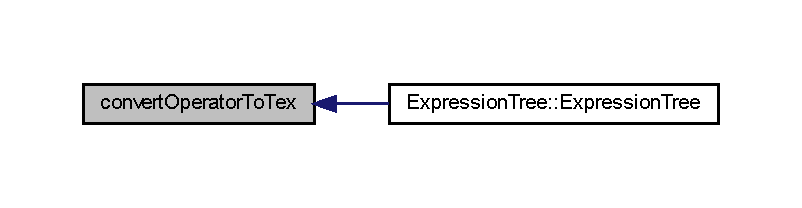
\includegraphics[width=350pt]{_convert_to_t_e_x_8cpp_ad4e5f83764391b1e3f08c01e12f84057_icgraph}
\end{center}
\end{figure}
\mbox{\Hypertarget{_convert_to_t_e_x_8cpp_a712748de4d9b72d7f5ee8c9bae5554b3}\label{_convert_to_t_e_x_8cpp_a712748de4d9b72d7f5ee8c9bae5554b3}} 
\index{Convert\+To\+T\+E\+X.\+cpp@{Convert\+To\+T\+E\+X.\+cpp}!get\+Priority\+Of\+Operator@{get\+Priority\+Of\+Operator}}
\index{get\+Priority\+Of\+Operator@{get\+Priority\+Of\+Operator}!Convert\+To\+T\+E\+X.\+cpp@{Convert\+To\+T\+E\+X.\+cpp}}
\subsubsection{\texorpdfstring{get\+Priority\+Of\+Operator()}{getPriorityOfOperator()}}
{\footnotesize\ttfamily int get\+Priority\+Of\+Operator (\begin{DoxyParamCaption}\item[{const string \&}]{str }\end{DoxyParamCaption})}



Определяпет приоритет оператора 


\begin{DoxyParams}[1]{Аргументы}
\mbox{\tt in}  & {\em str} & -\/ строка \\
\hline
\end{DoxyParams}
\begin{DoxyReturn}{Возвращает}
-\/ если строка является оператором, то приоритет оператора, иначе -\/1 
\end{DoxyReturn}
Граф вызова функции\+:\nopagebreak
\begin{figure}[H]
\begin{center}
\leavevmode
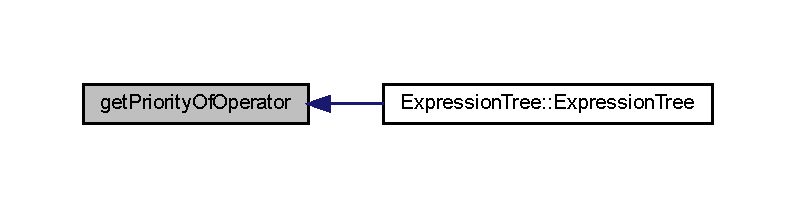
\includegraphics[width=350pt]{_convert_to_t_e_x_8cpp_a712748de4d9b72d7f5ee8c9bae5554b3_icgraph}
\end{center}
\end{figure}
\mbox{\Hypertarget{_convert_to_t_e_x_8cpp_ae21b6302b60f99394bf6855459a07953}\label{_convert_to_t_e_x_8cpp_ae21b6302b60f99394bf6855459a07953}} 
\index{Convert\+To\+T\+E\+X.\+cpp@{Convert\+To\+T\+E\+X.\+cpp}!handle\+Exceptions@{handle\+Exceptions}}
\index{handle\+Exceptions@{handle\+Exceptions}!Convert\+To\+T\+E\+X.\+cpp@{Convert\+To\+T\+E\+X.\+cpp}}
\subsubsection{\texorpdfstring{handle\+Exceptions()}{handleExceptions()}}
{\footnotesize\ttfamily void handle\+Exceptions (\begin{DoxyParamCaption}\item[{\mbox{\hyperlink{_convert_to_t_e_x_8h_a8852f03cd91327c7c725673317d85b46}{Exception}}}]{exception }\end{DoxyParamCaption})}



Обработать ошибку 


\begin{DoxyParams}[1]{Аргументы}
\mbox{\tt in}  & {\em exception} & -\/ исключение \\
\hline
\end{DoxyParams}
Граф вызова функции\+:\nopagebreak
\begin{figure}[H]
\begin{center}
\leavevmode
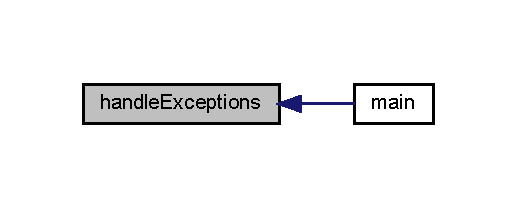
\includegraphics[width=248pt]{_convert_to_t_e_x_8cpp_ae21b6302b60f99394bf6855459a07953_icgraph}
\end{center}
\end{figure}
\mbox{\Hypertarget{_convert_to_t_e_x_8cpp_aa8d111bf48d55bf484f25b645680684d}\label{_convert_to_t_e_x_8cpp_aa8d111bf48d55bf484f25b645680684d}} 
\index{Convert\+To\+T\+E\+X.\+cpp@{Convert\+To\+T\+E\+X.\+cpp}!is\+Greek\+Letter@{is\+Greek\+Letter}}
\index{is\+Greek\+Letter@{is\+Greek\+Letter}!Convert\+To\+T\+E\+X.\+cpp@{Convert\+To\+T\+E\+X.\+cpp}}
\subsubsection{\texorpdfstring{is\+Greek\+Letter()}{isGreekLetter()}}
{\footnotesize\ttfamily bool is\+Greek\+Letter (\begin{DoxyParamCaption}\item[{const string \&}]{str }\end{DoxyParamCaption})}



Определяет, является ли строка греческой буквой 


\begin{DoxyParams}[1]{Аргументы}
\mbox{\tt in}  & {\em str} & -\/ строка \\
\hline
\end{DoxyParams}
\begin{DoxyReturn}{Возвращает}
-\/ если строка ялвяется греческой буквой, то true, иначе false 
\end{DoxyReturn}
Граф вызовов\+:\nopagebreak
\begin{figure}[H]
\begin{center}
\leavevmode
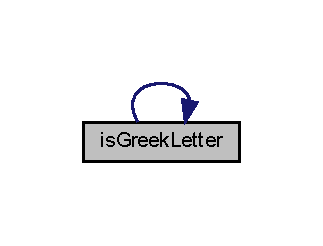
\includegraphics[width=155pt]{_convert_to_t_e_x_8cpp_aa8d111bf48d55bf484f25b645680684d_cgraph}
\end{center}
\end{figure}
Граф вызова функции\+:\nopagebreak
\begin{figure}[H]
\begin{center}
\leavevmode
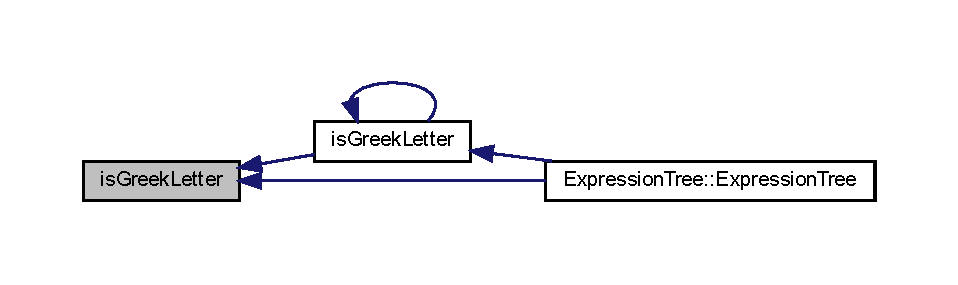
\includegraphics[width=350pt]{_convert_to_t_e_x_8cpp_aa8d111bf48d55bf484f25b645680684d_icgraph}
\end{center}
\end{figure}
\mbox{\Hypertarget{_convert_to_t_e_x_8cpp_a32365e377c80c8e22cf61b4f94ae1b02}\label{_convert_to_t_e_x_8cpp_a32365e377c80c8e22cf61b4f94ae1b02}} 
\index{Convert\+To\+T\+E\+X.\+cpp@{Convert\+To\+T\+E\+X.\+cpp}!is\+Number@{is\+Number}}
\index{is\+Number@{is\+Number}!Convert\+To\+T\+E\+X.\+cpp@{Convert\+To\+T\+E\+X.\+cpp}}
\subsubsection{\texorpdfstring{is\+Number()}{isNumber()}}
{\footnotesize\ttfamily bool is\+Number (\begin{DoxyParamCaption}\item[{const string \&}]{str }\end{DoxyParamCaption})}



Определяет, является ли строка числом 


\begin{DoxyParams}[1]{Аргументы}
\mbox{\tt in}  & {\em str} & -\/ строка \\
\hline
\end{DoxyParams}
\begin{DoxyReturn}{Возвращает}
-\/ если строка ялвяется числом, то true, иначе false 
\end{DoxyReturn}
Граф вызовов\+:\nopagebreak
\begin{figure}[H]
\begin{center}
\leavevmode
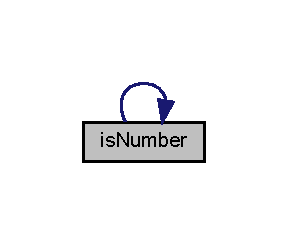
\includegraphics[width=138pt]{_convert_to_t_e_x_8cpp_a32365e377c80c8e22cf61b4f94ae1b02_cgraph}
\end{center}
\end{figure}
Граф вызова функции\+:\nopagebreak
\begin{figure}[H]
\begin{center}
\leavevmode
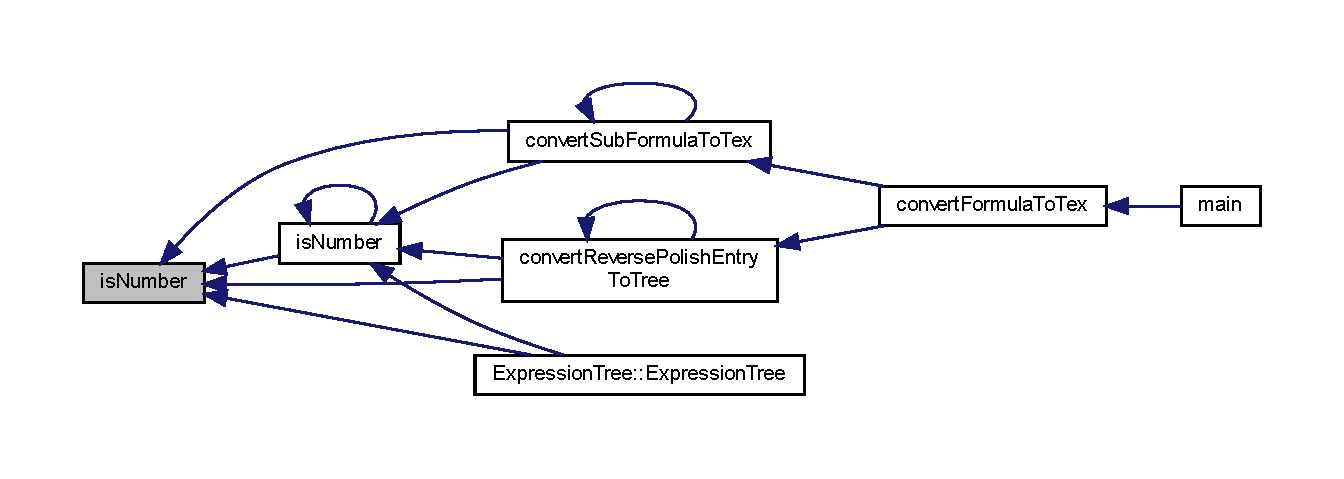
\includegraphics[width=350pt]{_convert_to_t_e_x_8cpp_a32365e377c80c8e22cf61b4f94ae1b02_icgraph}
\end{center}
\end{figure}
\mbox{\Hypertarget{_convert_to_t_e_x_8cpp_ac2b336cc6cd1fed67a0caf3f6f85a017}\label{_convert_to_t_e_x_8cpp_ac2b336cc6cd1fed67a0caf3f6f85a017}} 
\index{Convert\+To\+T\+E\+X.\+cpp@{Convert\+To\+T\+E\+X.\+cpp}!is\+Operator@{is\+Operator}}
\index{is\+Operator@{is\+Operator}!Convert\+To\+T\+E\+X.\+cpp@{Convert\+To\+T\+E\+X.\+cpp}}
\subsubsection{\texorpdfstring{is\+Operator()}{isOperator()}}
{\footnotesize\ttfamily int is\+Operator (\begin{DoxyParamCaption}\item[{const string \&}]{str }\end{DoxyParamCaption})}



Определяет, является ли строка оператором 


\begin{DoxyParams}[1]{Аргументы}
\mbox{\tt in}  & {\em str} & -\/ строка \\
\hline
\end{DoxyParams}
\begin{DoxyReturn}{Возвращает}
-\/ если строка ялвяется оператором, то количество операндов, иначе -\/1 
\end{DoxyReturn}
Граф вызова функции\+:\nopagebreak
\begin{figure}[H]
\begin{center}
\leavevmode
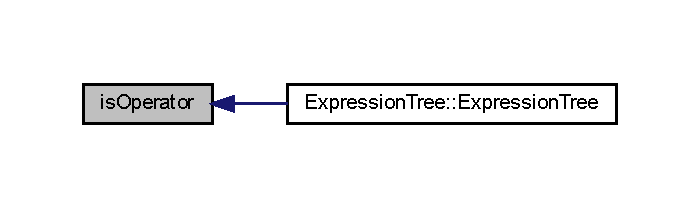
\includegraphics[width=336pt]{_convert_to_t_e_x_8cpp_ac2b336cc6cd1fed67a0caf3f6f85a017_icgraph}
\end{center}
\end{figure}
\mbox{\Hypertarget{_convert_to_t_e_x_8cpp_a7b85e910c81b100b63b513f076236ed9}\label{_convert_to_t_e_x_8cpp_a7b85e910c81b100b63b513f076236ed9}} 
\index{Convert\+To\+T\+E\+X.\+cpp@{Convert\+To\+T\+E\+X.\+cpp}!is\+Var@{is\+Var}}
\index{is\+Var@{is\+Var}!Convert\+To\+T\+E\+X.\+cpp@{Convert\+To\+T\+E\+X.\+cpp}}
\subsubsection{\texorpdfstring{is\+Var()}{isVar()}}
{\footnotesize\ttfamily bool is\+Var (\begin{DoxyParamCaption}\item[{const string \&}]{str }\end{DoxyParamCaption})}



Определяет, является ли строка переменной 


\begin{DoxyParams}[1]{Аргументы}
\mbox{\tt in}  & {\em str} & -\/ строка \\
\hline
\end{DoxyParams}
\begin{DoxyReturn}{Возвращает}
-\/ если строка является переменной, то true, иначе false 
\end{DoxyReturn}
Граф вызовов\+:\nopagebreak
\begin{figure}[H]
\begin{center}
\leavevmode
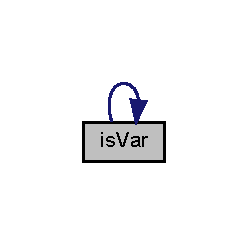
\includegraphics[width=119pt]{_convert_to_t_e_x_8cpp_a7b85e910c81b100b63b513f076236ed9_cgraph}
\end{center}
\end{figure}
Граф вызова функции\+:\nopagebreak
\begin{figure}[H]
\begin{center}
\leavevmode
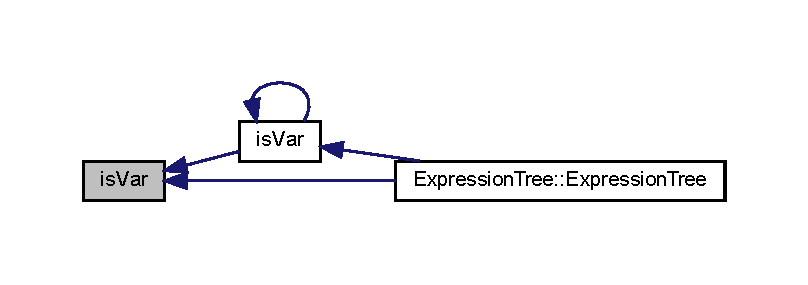
\includegraphics[width=350pt]{_convert_to_t_e_x_8cpp_a7b85e910c81b100b63b513f076236ed9_icgraph}
\end{center}
\end{figure}
\mbox{\Hypertarget{_convert_to_t_e_x_8cpp_aec4860ea778e9faaa79caa2f1e3a533e}\label{_convert_to_t_e_x_8cpp_aec4860ea778e9faaa79caa2f1e3a533e}} 
\index{Convert\+To\+T\+E\+X.\+cpp@{Convert\+To\+T\+E\+X.\+cpp}!read\+File@{read\+File}}
\index{read\+File@{read\+File}!Convert\+To\+T\+E\+X.\+cpp@{Convert\+To\+T\+E\+X.\+cpp}}
\subsubsection{\texorpdfstring{read\+File()}{readFile()}}
{\footnotesize\ttfamily void read\+File (\begin{DoxyParamCaption}\item[{string \&}]{file\+Name,  }\item[{string \&}]{reverse\+Polish\+Entry }\end{DoxyParamCaption})}



Прочитать содержимое файла 


\begin{DoxyParams}[1]{Аргументы}
\mbox{\tt in}  & {\em file\+Name} & -\/ имя входного файла \\
\hline
\mbox{\tt out}  & {\em reverse\+Polish\+Entry} & -\/ обратная польская запись \\
\hline
\end{DoxyParams}

\begin{DoxyExceptions}{Исключения}
{\em I\+N\+C\+O\+R\+R\+E\+C\+T\+\_\+\+E\+X\+T\+E\+N\+S\+I\+O\+N\+\_\+\+E\+X\+C\+E\+P\+T\+I\+ON} & -\/ файл имеет неверное расширение \\
\hline
{\em F\+I\+L\+E\+\_\+\+I\+N\+\_\+\+N\+O\+T\+\_\+\+F\+O\+U\+N\+D\+\_\+\+E\+X\+C\+E\+P\+T\+I\+ON} & -\/ файл не найден \\
\hline
{\em E\+M\+P\+T\+Y\+\_\+\+S\+T\+R\+I\+N\+G\+\_\+\+E\+X\+C\+E\+P\+T\+I\+ON} & -\/ файл содержит пустую строку \\
\hline
\end{DoxyExceptions}
Граф вызова функции\+:\nopagebreak
\begin{figure}[H]
\begin{center}
\leavevmode
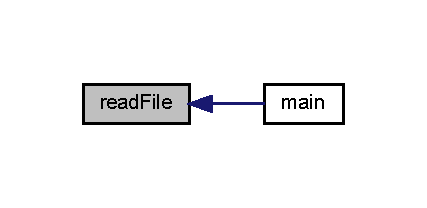
\includegraphics[width=205pt]{_convert_to_t_e_x_8cpp_aec4860ea778e9faaa79caa2f1e3a533e_icgraph}
\end{center}
\end{figure}
\mbox{\Hypertarget{_convert_to_t_e_x_8cpp_a705dee56a937b1f4d306aa1daf4a01b6}\label{_convert_to_t_e_x_8cpp_a705dee56a937b1f4d306aa1daf4a01b6}} 
\index{Convert\+To\+T\+E\+X.\+cpp@{Convert\+To\+T\+E\+X.\+cpp}!write\+To\+File@{write\+To\+File}}
\index{write\+To\+File@{write\+To\+File}!Convert\+To\+T\+E\+X.\+cpp@{Convert\+To\+T\+E\+X.\+cpp}}
\subsubsection{\texorpdfstring{write\+To\+File()}{writeToFile()}}
{\footnotesize\ttfamily void write\+To\+File (\begin{DoxyParamCaption}\item[{string \&}]{file\+Name,  }\item[{string \&}]{tex\+Formula }\end{DoxyParamCaption})}



Записать в файл 


\begin{DoxyParams}[1]{Аргументы}
\mbox{\tt in}  & {\em file\+Name} & -\/ имя выходного файла \\
\hline
\mbox{\tt in}  & {\em tex\+Formula} & -\/ tex-\/формула, которую мы должны записать в файл \\
\hline
\end{DoxyParams}
Граф вызова функции\+:\nopagebreak
\begin{figure}[H]
\begin{center}
\leavevmode
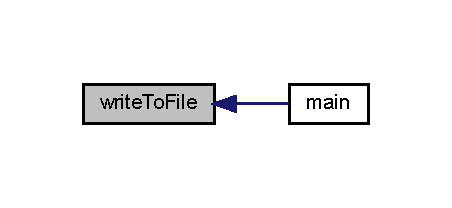
\includegraphics[width=217pt]{_convert_to_t_e_x_8cpp_a705dee56a937b1f4d306aa1daf4a01b6_icgraph}
\end{center}
\end{figure}

\hypertarget{_convert_to_t_e_x_8h}{}\section{Файл Convert\+To\+T\+E\+X.\+h}
\label{_convert_to_t_e_x_8h}\index{Convert\+To\+T\+E\+X.\+h@{Convert\+To\+T\+E\+X.\+h}}


Заголовочный файл с заголовками вспомогательных функций, а также перечисление исключений  


{\ttfamily \#include $<$iostream$>$}\newline
{\ttfamily \#include $<$vector$>$}\newline
{\ttfamily \#include $<$map$>$}\newline
\subsection*{Макросы}
\begin{DoxyCompactItemize}
\item 
\#define \mbox{\hyperlink{_convert_to_t_e_x_8h_af08ec37a8c99d747fb60fa15bc28678b}{\+\_\+\+C\+R\+T\+\_\+\+S\+E\+C\+U\+R\+E\+\_\+\+N\+O\+\_\+\+W\+A\+R\+N\+I\+N\+GS}}
\end{DoxyCompactItemize}
\subsection*{Перечисления}
\begin{DoxyCompactItemize}
\item 
enum \mbox{\hyperlink{_convert_to_t_e_x_8h_a8852f03cd91327c7c725673317d85b46}{Exception}} \{ \newline
\mbox{\hyperlink{_convert_to_t_e_x_8h_a8852f03cd91327c7c725673317d85b46ac7b69f92bbc35da9c437977199abed7e}{E\+M\+P\+T\+Y\+\_\+\+S\+T\+R\+I\+N\+G\+\_\+\+E\+X\+C\+E\+P\+T\+I\+ON}}, 
\mbox{\hyperlink{_convert_to_t_e_x_8h_a8852f03cd91327c7c725673317d85b46acae1b056d543cb9e6012ef2f57e09109}{F\+I\+L\+E\+\_\+\+I\+N\+\_\+\+N\+O\+T\+\_\+\+F\+O\+U\+N\+D\+\_\+\+E\+X\+C\+E\+P\+T\+I\+ON}}, 
\mbox{\hyperlink{_convert_to_t_e_x_8h_a8852f03cd91327c7c725673317d85b46a2c7eb3179e721e0aff0bbd39bb1fafea}{I\+N\+C\+O\+R\+R\+E\+C\+T\+\_\+\+E\+X\+T\+E\+N\+S\+I\+O\+N\+\_\+\+E\+X\+C\+E\+P\+T\+I\+ON}}, 
\mbox{\hyperlink{_convert_to_t_e_x_8h_a8852f03cd91327c7c725673317d85b46a7f391bb9e271a60ffbcf7799e6d779f0}{I\+N\+C\+O\+R\+R\+E\+C\+T\+\_\+\+V\+A\+L\+\_\+\+F\+O\+R\+M\+A\+T\+\_\+\+E\+X\+C\+E\+P\+T\+I\+ON}}, 
\newline
\mbox{\hyperlink{_convert_to_t_e_x_8h_a8852f03cd91327c7c725673317d85b46ae0440bca34f33370169dd37195a4ec1b}{I\+N\+C\+O\+R\+R\+E\+C\+T\+\_\+\+D\+I\+A\+P\+O\+S\+O\+N\+\_\+\+E\+X\+C\+E\+P\+T\+I\+ON}}, 
\mbox{\hyperlink{_convert_to_t_e_x_8h_a8852f03cd91327c7c725673317d85b46ab7d4a5f69539017907633cfcd8f970a8}{E\+X\+C\+E\+S\+S\+\_\+\+O\+F\+\_\+\+O\+P\+E\+R\+A\+N\+D\+S\+\_\+\+E\+X\+C\+E\+P\+T\+I\+ON}}, 
\mbox{\hyperlink{_convert_to_t_e_x_8h_a8852f03cd91327c7c725673317d85b46a77fd75de835d301f44563139eec339b3}{L\+A\+C\+K\+\_\+\+O\+F\+\_\+\+O\+P\+E\+R\+A\+N\+D\+S\+\_\+\+E\+X\+C\+E\+P\+T\+I\+ON}}, 
\mbox{\hyperlink{_convert_to_t_e_x_8h_a8852f03cd91327c7c725673317d85b46a3c8b6fc04207707cecbb1dbce7bfb00d}{L\+A\+C\+K\+\_\+\+O\+F\+\_\+\+C\+O\+N\+S\+O\+L\+E\+\_\+\+A\+R\+G\+U\+M\+E\+NT}}, 
\newline
\mbox{\hyperlink{_convert_to_t_e_x_8h_a8852f03cd91327c7c725673317d85b46a4b230c9962f4c95b0289ca90f893a3bc}{I\+N\+C\+O\+R\+R\+E\+C\+T\+\_\+\+E\+X\+T\+E\+N\+S\+I\+O\+N\+\_\+\+O\+U\+T\+P\+U\+T\+\_\+\+E\+X\+C\+E\+P\+T\+I\+ON}}, 
\mbox{\hyperlink{_convert_to_t_e_x_8h_a8852f03cd91327c7c725673317d85b46a1918b005c3a338a2b213077aeb2ffa03}{U\+N\+K\+N\+O\+W\+N\+\_\+\+E\+X\+C\+E\+P\+T\+I\+ON}}
 \}
\begin{DoxyCompactList}\small\item\em Перечисление ошибок \end{DoxyCompactList}\end{DoxyCompactItemize}
\subsection*{Функции}
\begin{DoxyCompactItemize}
\item 
bool \mbox{\hyperlink{_convert_to_t_e_x_8h_a7b85e910c81b100b63b513f076236ed9}{is\+Var}} (const string \&str)
\begin{DoxyCompactList}\small\item\em Определяет, является ли строка переменной \end{DoxyCompactList}\item 
bool \mbox{\hyperlink{_convert_to_t_e_x_8h_a32365e377c80c8e22cf61b4f94ae1b02}{is\+Number}} (const string \&str)
\begin{DoxyCompactList}\small\item\em Определяет, является ли строка числом \end{DoxyCompactList}\item 
bool \mbox{\hyperlink{_convert_to_t_e_x_8h_aa8d111bf48d55bf484f25b645680684d}{is\+Greek\+Letter}} (const string \&str)
\begin{DoxyCompactList}\small\item\em Определяет, является ли строка греческой буквой \end{DoxyCompactList}\item 
int \mbox{\hyperlink{_convert_to_t_e_x_8h_ac2b336cc6cd1fed67a0caf3f6f85a017}{is\+Operator}} (const string \&str)
\begin{DoxyCompactList}\small\item\em Определяет, является ли строка оператором \end{DoxyCompactList}\item 
int \mbox{\hyperlink{_convert_to_t_e_x_8h_a712748de4d9b72d7f5ee8c9bae5554b3}{get\+Priority\+Of\+Operator}} (const string \&str)
\begin{DoxyCompactList}\small\item\em Определяпет приоритет оператора \end{DoxyCompactList}\item 
void \mbox{\hyperlink{_convert_to_t_e_x_8h_ae21b6302b60f99394bf6855459a07953}{handle\+Exceptions}} (\mbox{\hyperlink{_convert_to_t_e_x_8h_a8852f03cd91327c7c725673317d85b46}{Exception}} exception)
\begin{DoxyCompactList}\small\item\em Обработать ошибку \end{DoxyCompactList}\item 
string \mbox{\hyperlink{_convert_to_t_e_x_8h_ad4e5f83764391b1e3f08c01e12f84057}{convert\+Operator\+To\+Tex}} (const string \&str)
\begin{DoxyCompactList}\small\item\em Конвертировать оператор из C-\/формата в tex-\/формат \end{DoxyCompactList}\item 
void \mbox{\hyperlink{_convert_to_t_e_x_8h_aec4860ea778e9faaa79caa2f1e3a533e}{read\+File}} (string \&file\+Name, string \&reverse\+Polish\+Entry)
\begin{DoxyCompactList}\small\item\em Прочитать содержимое файла \end{DoxyCompactList}\item 
void \mbox{\hyperlink{_convert_to_t_e_x_8h_a705dee56a937b1f4d306aa1daf4a01b6}{write\+To\+File}} (string \&file\+Name, string \&tex\+Formula)
\begin{DoxyCompactList}\small\item\em Записать в файл \end{DoxyCompactList}\end{DoxyCompactItemize}
\subsection*{Переменные}
\begin{DoxyCompactItemize}
\item 
const int \mbox{\hyperlink{_convert_to_t_e_x_8h_aaac987431c70181d544ce9ab8fb71aa3}{M\+A\+X\+\_\+\+O\+P\+E\+R\+A\+N\+D\+\_\+\+C\+O\+U\+NT}} = 3
\begin{DoxyCompactList}\small\item\em Максимальное количество операндов оператора \end{DoxyCompactList}\end{DoxyCompactItemize}


\subsection{Подробное описание}
Заголовочный файл с заголовками вспомогательных функций, а также перечисление исключений 

Данный файл содержит заголовки функций, необходимых для идентификации элемента обратной польской записи, чтение и записи в файл, функцию обработки ошибок, определение параметров оператора в обратной польской записи, а также перечисление исключений 

\subsection{Макросы}
\mbox{\Hypertarget{_convert_to_t_e_x_8h_af08ec37a8c99d747fb60fa15bc28678b}\label{_convert_to_t_e_x_8h_af08ec37a8c99d747fb60fa15bc28678b}} 
\index{Convert\+To\+T\+E\+X.\+h@{Convert\+To\+T\+E\+X.\+h}!\+\_\+\+C\+R\+T\+\_\+\+S\+E\+C\+U\+R\+E\+\_\+\+N\+O\+\_\+\+W\+A\+R\+N\+I\+N\+GS@{\+\_\+\+C\+R\+T\+\_\+\+S\+E\+C\+U\+R\+E\+\_\+\+N\+O\+\_\+\+W\+A\+R\+N\+I\+N\+GS}}
\index{\+\_\+\+C\+R\+T\+\_\+\+S\+E\+C\+U\+R\+E\+\_\+\+N\+O\+\_\+\+W\+A\+R\+N\+I\+N\+GS@{\+\_\+\+C\+R\+T\+\_\+\+S\+E\+C\+U\+R\+E\+\_\+\+N\+O\+\_\+\+W\+A\+R\+N\+I\+N\+GS}!Convert\+To\+T\+E\+X.\+h@{Convert\+To\+T\+E\+X.\+h}}
\subsubsection{\texorpdfstring{\+\_\+\+C\+R\+T\+\_\+\+S\+E\+C\+U\+R\+E\+\_\+\+N\+O\+\_\+\+W\+A\+R\+N\+I\+N\+GS}{\_CRT\_SECURE\_NO\_WARNINGS}}
{\footnotesize\ttfamily \#define \+\_\+\+C\+R\+T\+\_\+\+S\+E\+C\+U\+R\+E\+\_\+\+N\+O\+\_\+\+W\+A\+R\+N\+I\+N\+GS}



\subsection{Перечисления}
\mbox{\Hypertarget{_convert_to_t_e_x_8h_a8852f03cd91327c7c725673317d85b46}\label{_convert_to_t_e_x_8h_a8852f03cd91327c7c725673317d85b46}} 
\index{Convert\+To\+T\+E\+X.\+h@{Convert\+To\+T\+E\+X.\+h}!Exception@{Exception}}
\index{Exception@{Exception}!Convert\+To\+T\+E\+X.\+h@{Convert\+To\+T\+E\+X.\+h}}
\subsubsection{\texorpdfstring{Exception}{Exception}}
{\footnotesize\ttfamily enum \mbox{\hyperlink{_convert_to_t_e_x_8h_a8852f03cd91327c7c725673317d85b46}{Exception}}}



Перечисление ошибок 

\begin{DoxyEnumFields}{Элементы перечислений}
\raisebox{\heightof{T}}[0pt][0pt]{\index{E\+M\+P\+T\+Y\+\_\+\+S\+T\+R\+I\+N\+G\+\_\+\+E\+X\+C\+E\+P\+T\+I\+ON@{E\+M\+P\+T\+Y\+\_\+\+S\+T\+R\+I\+N\+G\+\_\+\+E\+X\+C\+E\+P\+T\+I\+ON}!Convert\+To\+T\+E\+X.\+h@{Convert\+To\+T\+E\+X.\+h}}\index{Convert\+To\+T\+E\+X.\+h@{Convert\+To\+T\+E\+X.\+h}!E\+M\+P\+T\+Y\+\_\+\+S\+T\+R\+I\+N\+G\+\_\+\+E\+X\+C\+E\+P\+T\+I\+ON@{E\+M\+P\+T\+Y\+\_\+\+S\+T\+R\+I\+N\+G\+\_\+\+E\+X\+C\+E\+P\+T\+I\+ON}}}\mbox{\Hypertarget{_convert_to_t_e_x_8h_a8852f03cd91327c7c725673317d85b46ac7b69f92bbc35da9c437977199abed7e}\label{_convert_to_t_e_x_8h_a8852f03cd91327c7c725673317d85b46ac7b69f92bbc35da9c437977199abed7e}} 
E\+M\+P\+T\+Y\+\_\+\+S\+T\+R\+I\+N\+G\+\_\+\+E\+X\+C\+E\+P\+T\+I\+ON&Пустая строка \\
\hline

\raisebox{\heightof{T}}[0pt][0pt]{\index{F\+I\+L\+E\+\_\+\+I\+N\+\_\+\+N\+O\+T\+\_\+\+F\+O\+U\+N\+D\+\_\+\+E\+X\+C\+E\+P\+T\+I\+ON@{F\+I\+L\+E\+\_\+\+I\+N\+\_\+\+N\+O\+T\+\_\+\+F\+O\+U\+N\+D\+\_\+\+E\+X\+C\+E\+P\+T\+I\+ON}!Convert\+To\+T\+E\+X.\+h@{Convert\+To\+T\+E\+X.\+h}}\index{Convert\+To\+T\+E\+X.\+h@{Convert\+To\+T\+E\+X.\+h}!F\+I\+L\+E\+\_\+\+I\+N\+\_\+\+N\+O\+T\+\_\+\+F\+O\+U\+N\+D\+\_\+\+E\+X\+C\+E\+P\+T\+I\+ON@{F\+I\+L\+E\+\_\+\+I\+N\+\_\+\+N\+O\+T\+\_\+\+F\+O\+U\+N\+D\+\_\+\+E\+X\+C\+E\+P\+T\+I\+ON}}}\mbox{\Hypertarget{_convert_to_t_e_x_8h_a8852f03cd91327c7c725673317d85b46acae1b056d543cb9e6012ef2f57e09109}\label{_convert_to_t_e_x_8h_a8852f03cd91327c7c725673317d85b46acae1b056d543cb9e6012ef2f57e09109}} 
F\+I\+L\+E\+\_\+\+I\+N\+\_\+\+N\+O\+T\+\_\+\+F\+O\+U\+N\+D\+\_\+\+E\+X\+C\+E\+P\+T\+I\+ON&Файл c входными данными не найден \\
\hline

\raisebox{\heightof{T}}[0pt][0pt]{\index{I\+N\+C\+O\+R\+R\+E\+C\+T\+\_\+\+E\+X\+T\+E\+N\+S\+I\+O\+N\+\_\+\+E\+X\+C\+E\+P\+T\+I\+ON@{I\+N\+C\+O\+R\+R\+E\+C\+T\+\_\+\+E\+X\+T\+E\+N\+S\+I\+O\+N\+\_\+\+E\+X\+C\+E\+P\+T\+I\+ON}!Convert\+To\+T\+E\+X.\+h@{Convert\+To\+T\+E\+X.\+h}}\index{Convert\+To\+T\+E\+X.\+h@{Convert\+To\+T\+E\+X.\+h}!I\+N\+C\+O\+R\+R\+E\+C\+T\+\_\+\+E\+X\+T\+E\+N\+S\+I\+O\+N\+\_\+\+E\+X\+C\+E\+P\+T\+I\+ON@{I\+N\+C\+O\+R\+R\+E\+C\+T\+\_\+\+E\+X\+T\+E\+N\+S\+I\+O\+N\+\_\+\+E\+X\+C\+E\+P\+T\+I\+ON}}}\mbox{\Hypertarget{_convert_to_t_e_x_8h_a8852f03cd91327c7c725673317d85b46a2c7eb3179e721e0aff0bbd39bb1fafea}\label{_convert_to_t_e_x_8h_a8852f03cd91327c7c725673317d85b46a2c7eb3179e721e0aff0bbd39bb1fafea}} 
I\+N\+C\+O\+R\+R\+E\+C\+T\+\_\+\+E\+X\+T\+E\+N\+S\+I\+O\+N\+\_\+\+E\+X\+C\+E\+P\+T\+I\+ON&Неверное расширение файла \\
\hline

\raisebox{\heightof{T}}[0pt][0pt]{\index{I\+N\+C\+O\+R\+R\+E\+C\+T\+\_\+\+V\+A\+L\+\_\+\+F\+O\+R\+M\+A\+T\+\_\+\+E\+X\+C\+E\+P\+T\+I\+ON@{I\+N\+C\+O\+R\+R\+E\+C\+T\+\_\+\+V\+A\+L\+\_\+\+F\+O\+R\+M\+A\+T\+\_\+\+E\+X\+C\+E\+P\+T\+I\+ON}!Convert\+To\+T\+E\+X.\+h@{Convert\+To\+T\+E\+X.\+h}}\index{Convert\+To\+T\+E\+X.\+h@{Convert\+To\+T\+E\+X.\+h}!I\+N\+C\+O\+R\+R\+E\+C\+T\+\_\+\+V\+A\+L\+\_\+\+F\+O\+R\+M\+A\+T\+\_\+\+E\+X\+C\+E\+P\+T\+I\+ON@{I\+N\+C\+O\+R\+R\+E\+C\+T\+\_\+\+V\+A\+L\+\_\+\+F\+O\+R\+M\+A\+T\+\_\+\+E\+X\+C\+E\+P\+T\+I\+ON}}}\mbox{\Hypertarget{_convert_to_t_e_x_8h_a8852f03cd91327c7c725673317d85b46a7f391bb9e271a60ffbcf7799e6d779f0}\label{_convert_to_t_e_x_8h_a8852f03cd91327c7c725673317d85b46a7f391bb9e271a60ffbcf7799e6d779f0}} 
I\+N\+C\+O\+R\+R\+E\+C\+T\+\_\+\+V\+A\+L\+\_\+\+F\+O\+R\+M\+A\+T\+\_\+\+E\+X\+C\+E\+P\+T\+I\+ON&Неверный формат для элемента обратной польской записи \\
\hline

\raisebox{\heightof{T}}[0pt][0pt]{\index{I\+N\+C\+O\+R\+R\+E\+C\+T\+\_\+\+D\+I\+A\+P\+O\+S\+O\+N\+\_\+\+E\+X\+C\+E\+P\+T\+I\+ON@{I\+N\+C\+O\+R\+R\+E\+C\+T\+\_\+\+D\+I\+A\+P\+O\+S\+O\+N\+\_\+\+E\+X\+C\+E\+P\+T\+I\+ON}!Convert\+To\+T\+E\+X.\+h@{Convert\+To\+T\+E\+X.\+h}}\index{Convert\+To\+T\+E\+X.\+h@{Convert\+To\+T\+E\+X.\+h}!I\+N\+C\+O\+R\+R\+E\+C\+T\+\_\+\+D\+I\+A\+P\+O\+S\+O\+N\+\_\+\+E\+X\+C\+E\+P\+T\+I\+ON@{I\+N\+C\+O\+R\+R\+E\+C\+T\+\_\+\+D\+I\+A\+P\+O\+S\+O\+N\+\_\+\+E\+X\+C\+E\+P\+T\+I\+ON}}}\mbox{\Hypertarget{_convert_to_t_e_x_8h_a8852f03cd91327c7c725673317d85b46ae0440bca34f33370169dd37195a4ec1b}\label{_convert_to_t_e_x_8h_a8852f03cd91327c7c725673317d85b46ae0440bca34f33370169dd37195a4ec1b}} 
I\+N\+C\+O\+R\+R\+E\+C\+T\+\_\+\+D\+I\+A\+P\+O\+S\+O\+N\+\_\+\+E\+X\+C\+E\+P\+T\+I\+ON&Неверный диапозон для чисел в обратной польской записи \\
\hline

\raisebox{\heightof{T}}[0pt][0pt]{\index{E\+X\+C\+E\+S\+S\+\_\+\+O\+F\+\_\+\+O\+P\+E\+R\+A\+N\+D\+S\+\_\+\+E\+X\+C\+E\+P\+T\+I\+ON@{E\+X\+C\+E\+S\+S\+\_\+\+O\+F\+\_\+\+O\+P\+E\+R\+A\+N\+D\+S\+\_\+\+E\+X\+C\+E\+P\+T\+I\+ON}!Convert\+To\+T\+E\+X.\+h@{Convert\+To\+T\+E\+X.\+h}}\index{Convert\+To\+T\+E\+X.\+h@{Convert\+To\+T\+E\+X.\+h}!E\+X\+C\+E\+S\+S\+\_\+\+O\+F\+\_\+\+O\+P\+E\+R\+A\+N\+D\+S\+\_\+\+E\+X\+C\+E\+P\+T\+I\+ON@{E\+X\+C\+E\+S\+S\+\_\+\+O\+F\+\_\+\+O\+P\+E\+R\+A\+N\+D\+S\+\_\+\+E\+X\+C\+E\+P\+T\+I\+ON}}}\mbox{\Hypertarget{_convert_to_t_e_x_8h_a8852f03cd91327c7c725673317d85b46ab7d4a5f69539017907633cfcd8f970a8}\label{_convert_to_t_e_x_8h_a8852f03cd91327c7c725673317d85b46ab7d4a5f69539017907633cfcd8f970a8}} 
E\+X\+C\+E\+S\+S\+\_\+\+O\+F\+\_\+\+O\+P\+E\+R\+A\+N\+D\+S\+\_\+\+E\+X\+C\+E\+P\+T\+I\+ON&Количество операндов больше необходимого \\
\hline

\raisebox{\heightof{T}}[0pt][0pt]{\index{L\+A\+C\+K\+\_\+\+O\+F\+\_\+\+O\+P\+E\+R\+A\+N\+D\+S\+\_\+\+E\+X\+C\+E\+P\+T\+I\+ON@{L\+A\+C\+K\+\_\+\+O\+F\+\_\+\+O\+P\+E\+R\+A\+N\+D\+S\+\_\+\+E\+X\+C\+E\+P\+T\+I\+ON}!Convert\+To\+T\+E\+X.\+h@{Convert\+To\+T\+E\+X.\+h}}\index{Convert\+To\+T\+E\+X.\+h@{Convert\+To\+T\+E\+X.\+h}!L\+A\+C\+K\+\_\+\+O\+F\+\_\+\+O\+P\+E\+R\+A\+N\+D\+S\+\_\+\+E\+X\+C\+E\+P\+T\+I\+ON@{L\+A\+C\+K\+\_\+\+O\+F\+\_\+\+O\+P\+E\+R\+A\+N\+D\+S\+\_\+\+E\+X\+C\+E\+P\+T\+I\+ON}}}\mbox{\Hypertarget{_convert_to_t_e_x_8h_a8852f03cd91327c7c725673317d85b46a77fd75de835d301f44563139eec339b3}\label{_convert_to_t_e_x_8h_a8852f03cd91327c7c725673317d85b46a77fd75de835d301f44563139eec339b3}} 
L\+A\+C\+K\+\_\+\+O\+F\+\_\+\+O\+P\+E\+R\+A\+N\+D\+S\+\_\+\+E\+X\+C\+E\+P\+T\+I\+ON&Количество операндов меньше необходимого \\
\hline

\raisebox{\heightof{T}}[0pt][0pt]{\index{L\+A\+C\+K\+\_\+\+O\+F\+\_\+\+C\+O\+N\+S\+O\+L\+E\+\_\+\+A\+R\+G\+U\+M\+E\+NT@{L\+A\+C\+K\+\_\+\+O\+F\+\_\+\+C\+O\+N\+S\+O\+L\+E\+\_\+\+A\+R\+G\+U\+M\+E\+NT}!Convert\+To\+T\+E\+X.\+h@{Convert\+To\+T\+E\+X.\+h}}\index{Convert\+To\+T\+E\+X.\+h@{Convert\+To\+T\+E\+X.\+h}!L\+A\+C\+K\+\_\+\+O\+F\+\_\+\+C\+O\+N\+S\+O\+L\+E\+\_\+\+A\+R\+G\+U\+M\+E\+NT@{L\+A\+C\+K\+\_\+\+O\+F\+\_\+\+C\+O\+N\+S\+O\+L\+E\+\_\+\+A\+R\+G\+U\+M\+E\+NT}}}\mbox{\Hypertarget{_convert_to_t_e_x_8h_a8852f03cd91327c7c725673317d85b46a3c8b6fc04207707cecbb1dbce7bfb00d}\label{_convert_to_t_e_x_8h_a8852f03cd91327c7c725673317d85b46a3c8b6fc04207707cecbb1dbce7bfb00d}} 
L\+A\+C\+K\+\_\+\+O\+F\+\_\+\+C\+O\+N\+S\+O\+L\+E\+\_\+\+A\+R\+G\+U\+M\+E\+NT&Количество аргументов консоли меньше необходимого \\
\hline

\raisebox{\heightof{T}}[0pt][0pt]{\index{I\+N\+C\+O\+R\+R\+E\+C\+T\+\_\+\+E\+X\+T\+E\+N\+S\+I\+O\+N\+\_\+\+O\+U\+T\+P\+U\+T\+\_\+\+E\+X\+C\+E\+P\+T\+I\+ON@{I\+N\+C\+O\+R\+R\+E\+C\+T\+\_\+\+E\+X\+T\+E\+N\+S\+I\+O\+N\+\_\+\+O\+U\+T\+P\+U\+T\+\_\+\+E\+X\+C\+E\+P\+T\+I\+ON}!Convert\+To\+T\+E\+X.\+h@{Convert\+To\+T\+E\+X.\+h}}\index{Convert\+To\+T\+E\+X.\+h@{Convert\+To\+T\+E\+X.\+h}!I\+N\+C\+O\+R\+R\+E\+C\+T\+\_\+\+E\+X\+T\+E\+N\+S\+I\+O\+N\+\_\+\+O\+U\+T\+P\+U\+T\+\_\+\+E\+X\+C\+E\+P\+T\+I\+ON@{I\+N\+C\+O\+R\+R\+E\+C\+T\+\_\+\+E\+X\+T\+E\+N\+S\+I\+O\+N\+\_\+\+O\+U\+T\+P\+U\+T\+\_\+\+E\+X\+C\+E\+P\+T\+I\+ON}}}\mbox{\Hypertarget{_convert_to_t_e_x_8h_a8852f03cd91327c7c725673317d85b46a4b230c9962f4c95b0289ca90f893a3bc}\label{_convert_to_t_e_x_8h_a8852f03cd91327c7c725673317d85b46a4b230c9962f4c95b0289ca90f893a3bc}} 
I\+N\+C\+O\+R\+R\+E\+C\+T\+\_\+\+E\+X\+T\+E\+N\+S\+I\+O\+N\+\_\+\+O\+U\+T\+P\+U\+T\+\_\+\+E\+X\+C\+E\+P\+T\+I\+ON&Неверное расширение выходного файла \\
\hline

\raisebox{\heightof{T}}[0pt][0pt]{\index{U\+N\+K\+N\+O\+W\+N\+\_\+\+E\+X\+C\+E\+P\+T\+I\+ON@{U\+N\+K\+N\+O\+W\+N\+\_\+\+E\+X\+C\+E\+P\+T\+I\+ON}!Convert\+To\+T\+E\+X.\+h@{Convert\+To\+T\+E\+X.\+h}}\index{Convert\+To\+T\+E\+X.\+h@{Convert\+To\+T\+E\+X.\+h}!U\+N\+K\+N\+O\+W\+N\+\_\+\+E\+X\+C\+E\+P\+T\+I\+ON@{U\+N\+K\+N\+O\+W\+N\+\_\+\+E\+X\+C\+E\+P\+T\+I\+ON}}}\mbox{\Hypertarget{_convert_to_t_e_x_8h_a8852f03cd91327c7c725673317d85b46a1918b005c3a338a2b213077aeb2ffa03}\label{_convert_to_t_e_x_8h_a8852f03cd91327c7c725673317d85b46a1918b005c3a338a2b213077aeb2ffa03}} 
U\+N\+K\+N\+O\+W\+N\+\_\+\+E\+X\+C\+E\+P\+T\+I\+ON&Неизвестное исключение \\
\hline

\end{DoxyEnumFields}


\subsection{Функции}
\mbox{\Hypertarget{_convert_to_t_e_x_8h_ad4e5f83764391b1e3f08c01e12f84057}\label{_convert_to_t_e_x_8h_ad4e5f83764391b1e3f08c01e12f84057}} 
\index{Convert\+To\+T\+E\+X.\+h@{Convert\+To\+T\+E\+X.\+h}!convert\+Operator\+To\+Tex@{convert\+Operator\+To\+Tex}}
\index{convert\+Operator\+To\+Tex@{convert\+Operator\+To\+Tex}!Convert\+To\+T\+E\+X.\+h@{Convert\+To\+T\+E\+X.\+h}}
\subsubsection{\texorpdfstring{convert\+Operator\+To\+Tex()}{convertOperatorToTex()}}
{\footnotesize\ttfamily string convert\+Operator\+To\+Tex (\begin{DoxyParamCaption}\item[{const string \&}]{str }\end{DoxyParamCaption})}



Конвертировать оператор из C-\/формата в tex-\/формат 


\begin{DoxyParams}[1]{Аргументы}
\mbox{\tt in}  & {\em str} & -\/ строка, являющаяся оператором \\
\hline
\end{DoxyParams}
\begin{DoxyReturn}{Возвращает}
-\/ оператор в tex-\/формате 
\end{DoxyReturn}
Граф вызова функции\+:
% FIG 0
\mbox{\Hypertarget{_convert_to_t_e_x_8h_a712748de4d9b72d7f5ee8c9bae5554b3}\label{_convert_to_t_e_x_8h_a712748de4d9b72d7f5ee8c9bae5554b3}} 
\index{Convert\+To\+T\+E\+X.\+h@{Convert\+To\+T\+E\+X.\+h}!get\+Priority\+Of\+Operator@{get\+Priority\+Of\+Operator}}
\index{get\+Priority\+Of\+Operator@{get\+Priority\+Of\+Operator}!Convert\+To\+T\+E\+X.\+h@{Convert\+To\+T\+E\+X.\+h}}
\subsubsection{\texorpdfstring{get\+Priority\+Of\+Operator()}{getPriorityOfOperator()}}
{\footnotesize\ttfamily int get\+Priority\+Of\+Operator (\begin{DoxyParamCaption}\item[{const string \&}]{str }\end{DoxyParamCaption})}



Определяпет приоритет оператора 


\begin{DoxyParams}[1]{Аргументы}
\mbox{\tt in}  & {\em str} & -\/ строка \\
\hline
\end{DoxyParams}
\begin{DoxyReturn}{Возвращает}
-\/ если строка является оператором, то приоритет оператора, иначе -\/1 
\end{DoxyReturn}
Граф вызова функции\+:
% FIG 1
\mbox{\Hypertarget{_convert_to_t_e_x_8h_ae21b6302b60f99394bf6855459a07953}\label{_convert_to_t_e_x_8h_ae21b6302b60f99394bf6855459a07953}} 
\index{Convert\+To\+T\+E\+X.\+h@{Convert\+To\+T\+E\+X.\+h}!handle\+Exceptions@{handle\+Exceptions}}
\index{handle\+Exceptions@{handle\+Exceptions}!Convert\+To\+T\+E\+X.\+h@{Convert\+To\+T\+E\+X.\+h}}
\subsubsection{\texorpdfstring{handle\+Exceptions()}{handleExceptions()}}
{\footnotesize\ttfamily void handle\+Exceptions (\begin{DoxyParamCaption}\item[{\mbox{\hyperlink{_convert_to_t_e_x_8h_a8852f03cd91327c7c725673317d85b46}{Exception}}}]{exception }\end{DoxyParamCaption})}



Обработать ошибку 


\begin{DoxyParams}[1]{Аргументы}
\mbox{\tt in}  & {\em exception} & -\/ исключение \\
\hline
\end{DoxyParams}
Граф вызова функции\+:
% FIG 2
\mbox{\Hypertarget{_convert_to_t_e_x_8h_aa8d111bf48d55bf484f25b645680684d}\label{_convert_to_t_e_x_8h_aa8d111bf48d55bf484f25b645680684d}} 
\index{Convert\+To\+T\+E\+X.\+h@{Convert\+To\+T\+E\+X.\+h}!is\+Greek\+Letter@{is\+Greek\+Letter}}
\index{is\+Greek\+Letter@{is\+Greek\+Letter}!Convert\+To\+T\+E\+X.\+h@{Convert\+To\+T\+E\+X.\+h}}
\subsubsection{\texorpdfstring{is\+Greek\+Letter()}{isGreekLetter()}}
{\footnotesize\ttfamily bool is\+Greek\+Letter (\begin{DoxyParamCaption}\item[{const string \&}]{str }\end{DoxyParamCaption})}



Определяет, является ли строка греческой буквой 


\begin{DoxyParams}[1]{Аргументы}
\mbox{\tt in}  & {\em str} & -\/ строка \\
\hline
\end{DoxyParams}
\begin{DoxyReturn}{Возвращает}
-\/ если строка ялвяется греческой буквой, то true, иначе false 
\end{DoxyReturn}
Граф вызовов\+:
% FIG 3
Граф вызова функции\+:
% FIG 4
\mbox{\Hypertarget{_convert_to_t_e_x_8h_a32365e377c80c8e22cf61b4f94ae1b02}\label{_convert_to_t_e_x_8h_a32365e377c80c8e22cf61b4f94ae1b02}} 
\index{Convert\+To\+T\+E\+X.\+h@{Convert\+To\+T\+E\+X.\+h}!is\+Number@{is\+Number}}
\index{is\+Number@{is\+Number}!Convert\+To\+T\+E\+X.\+h@{Convert\+To\+T\+E\+X.\+h}}
\subsubsection{\texorpdfstring{is\+Number()}{isNumber()}}
{\footnotesize\ttfamily bool is\+Number (\begin{DoxyParamCaption}\item[{const string \&}]{str }\end{DoxyParamCaption})}



Определяет, является ли строка числом 


\begin{DoxyParams}[1]{Аргументы}
\mbox{\tt in}  & {\em str} & -\/ строка \\
\hline
\end{DoxyParams}
\begin{DoxyReturn}{Возвращает}
-\/ если строка ялвяется числом, то true, иначе false 
\end{DoxyReturn}
Граф вызовов\+:
% FIG 5
Граф вызова функции\+:
% FIG 6
\mbox{\Hypertarget{_convert_to_t_e_x_8h_ac2b336cc6cd1fed67a0caf3f6f85a017}\label{_convert_to_t_e_x_8h_ac2b336cc6cd1fed67a0caf3f6f85a017}} 
\index{Convert\+To\+T\+E\+X.\+h@{Convert\+To\+T\+E\+X.\+h}!is\+Operator@{is\+Operator}}
\index{is\+Operator@{is\+Operator}!Convert\+To\+T\+E\+X.\+h@{Convert\+To\+T\+E\+X.\+h}}
\subsubsection{\texorpdfstring{is\+Operator()}{isOperator()}}
{\footnotesize\ttfamily int is\+Operator (\begin{DoxyParamCaption}\item[{const string \&}]{str }\end{DoxyParamCaption})}



Определяет, является ли строка оператором 


\begin{DoxyParams}[1]{Аргументы}
\mbox{\tt in}  & {\em str} & -\/ строка \\
\hline
\end{DoxyParams}
\begin{DoxyReturn}{Возвращает}
-\/ если строка ялвяется оператором, то количество операндов, иначе -\/1 
\end{DoxyReturn}
Граф вызова функции\+:
% FIG 7
\mbox{\Hypertarget{_convert_to_t_e_x_8h_a7b85e910c81b100b63b513f076236ed9}\label{_convert_to_t_e_x_8h_a7b85e910c81b100b63b513f076236ed9}} 
\index{Convert\+To\+T\+E\+X.\+h@{Convert\+To\+T\+E\+X.\+h}!is\+Var@{is\+Var}}
\index{is\+Var@{is\+Var}!Convert\+To\+T\+E\+X.\+h@{Convert\+To\+T\+E\+X.\+h}}
\subsubsection{\texorpdfstring{is\+Var()}{isVar()}}
{\footnotesize\ttfamily bool is\+Var (\begin{DoxyParamCaption}\item[{const string \&}]{str }\end{DoxyParamCaption})}



Определяет, является ли строка переменной 


\begin{DoxyParams}[1]{Аргументы}
\mbox{\tt in}  & {\em str} & -\/ строка \\
\hline
\end{DoxyParams}
\begin{DoxyReturn}{Возвращает}
-\/ если строка является переменной, то true, иначе false 
\end{DoxyReturn}
Граф вызовов\+:
% FIG 8
Граф вызова функции\+:
% FIG 9
\mbox{\Hypertarget{_convert_to_t_e_x_8h_aec4860ea778e9faaa79caa2f1e3a533e}\label{_convert_to_t_e_x_8h_aec4860ea778e9faaa79caa2f1e3a533e}} 
\index{Convert\+To\+T\+E\+X.\+h@{Convert\+To\+T\+E\+X.\+h}!read\+File@{read\+File}}
\index{read\+File@{read\+File}!Convert\+To\+T\+E\+X.\+h@{Convert\+To\+T\+E\+X.\+h}}
\subsubsection{\texorpdfstring{read\+File()}{readFile()}}
{\footnotesize\ttfamily void read\+File (\begin{DoxyParamCaption}\item[{string \&}]{file\+Name,  }\item[{string \&}]{reverse\+Polish\+Entry }\end{DoxyParamCaption})}



Прочитать содержимое файла 


\begin{DoxyParams}[1]{Аргументы}
\mbox{\tt in}  & {\em file\+Name} & -\/ имя входного файла \\
\hline
\mbox{\tt out}  & {\em reverse\+Polish\+Entry} & -\/ обратная польская запись \\
\hline
\end{DoxyParams}

\begin{DoxyExceptions}{Исключения}
{\em I\+N\+C\+O\+R\+R\+E\+C\+T\+\_\+\+E\+X\+T\+E\+N\+S\+I\+O\+N\+\_\+\+E\+X\+C\+E\+P\+T\+I\+ON} & -\/ файл имеет неверное расширение \\
\hline
{\em F\+I\+L\+E\+\_\+\+I\+N\+\_\+\+N\+O\+T\+\_\+\+F\+O\+U\+N\+D\+\_\+\+E\+X\+C\+E\+P\+T\+I\+ON} & -\/ файл не найден \\
\hline
{\em E\+M\+P\+T\+Y\+\_\+\+S\+T\+R\+I\+N\+G\+\_\+\+E\+X\+C\+E\+P\+T\+I\+ON} & -\/ файл содержит пустую строку \\
\hline
\end{DoxyExceptions}
Граф вызова функции\+:
% FIG 10
\mbox{\Hypertarget{_convert_to_t_e_x_8h_a705dee56a937b1f4d306aa1daf4a01b6}\label{_convert_to_t_e_x_8h_a705dee56a937b1f4d306aa1daf4a01b6}} 
\index{Convert\+To\+T\+E\+X.\+h@{Convert\+To\+T\+E\+X.\+h}!write\+To\+File@{write\+To\+File}}
\index{write\+To\+File@{write\+To\+File}!Convert\+To\+T\+E\+X.\+h@{Convert\+To\+T\+E\+X.\+h}}
\subsubsection{\texorpdfstring{write\+To\+File()}{writeToFile()}}
{\footnotesize\ttfamily void write\+To\+File (\begin{DoxyParamCaption}\item[{string \&}]{file\+Name,  }\item[{string \&}]{tex\+Formula }\end{DoxyParamCaption})}



Записать в файл 


\begin{DoxyParams}[1]{Аргументы}
\mbox{\tt in}  & {\em file\+Name} & -\/ имя выходного файла \\
\hline
\mbox{\tt in}  & {\em tex\+Formula} & -\/ tex-\/формула, которую мы должны записать в файл \\
\hline
\end{DoxyParams}
Граф вызова функции\+:
% FIG 11


\subsection{Переменные}
\mbox{\Hypertarget{_convert_to_t_e_x_8h_aaac987431c70181d544ce9ab8fb71aa3}\label{_convert_to_t_e_x_8h_aaac987431c70181d544ce9ab8fb71aa3}} 
\index{Convert\+To\+T\+E\+X.\+h@{Convert\+To\+T\+E\+X.\+h}!M\+A\+X\+\_\+\+O\+P\+E\+R\+A\+N\+D\+\_\+\+C\+O\+U\+NT@{M\+A\+X\+\_\+\+O\+P\+E\+R\+A\+N\+D\+\_\+\+C\+O\+U\+NT}}
\index{M\+A\+X\+\_\+\+O\+P\+E\+R\+A\+N\+D\+\_\+\+C\+O\+U\+NT@{M\+A\+X\+\_\+\+O\+P\+E\+R\+A\+N\+D\+\_\+\+C\+O\+U\+NT}!Convert\+To\+T\+E\+X.\+h@{Convert\+To\+T\+E\+X.\+h}}
\subsubsection{\texorpdfstring{M\+A\+X\+\_\+\+O\+P\+E\+R\+A\+N\+D\+\_\+\+C\+O\+U\+NT}{MAX\_OPERAND\_COUNT}}
{\footnotesize\ttfamily const int M\+A\+X\+\_\+\+O\+P\+E\+R\+A\+N\+D\+\_\+\+C\+O\+U\+NT = 3}



Максимальное количество операндов оператора 


\hypertarget{convert_tree_to_t_e_x_8cpp}{}\section{Файл convert\+Tree\+To\+T\+E\+X.\+cpp}
\label{convert_tree_to_t_e_x_8cpp}\index{convert\+Tree\+To\+T\+E\+X.\+cpp@{convert\+Tree\+To\+T\+E\+X.\+cpp}}


Файл содержит реализации функций перевода обратной польской записи в tex-\/Формулу, а также конвертация обратной пользской записи в дерево выражений  


{\ttfamily \#include \char`\"{}convert\+Tree\+To\+T\+E\+X.\+h\char`\"{}}\newline
{\ttfamily \#include $<$boost/algorithm/string.\+hpp$>$}\newline
{\ttfamily \#include $<$boost/regex.\+hpp$>$}\newline
{\ttfamily \#include \char`\"{}boost/lexical\+\_\+cast.\+hpp\char`\"{}}\newline
\subsection*{Функции}
\begin{DoxyCompactItemize}
\item 
\mbox{\hyperlink{class_expression_tree}{Expression\+Tree}} $\ast$ \mbox{\hyperlink{convert_tree_to_t_e_x_8cpp_a4484ae20417cae4ad61d6319cdf03f68}{convert\+Reverse\+Polish\+Entry\+To\+Tree}} (vector$<$ string $>$ \&reverse\+Polish\+Entry\+Elements)
\begin{DoxyCompactList}\small\item\em Конвертировать обратную польскую запись в дерево выражений \end{DoxyCompactList}\item 
string \mbox{\hyperlink{convert_tree_to_t_e_x_8cpp_acccbe3becd02b6dee976c55008082244}{convert\+Sub\+Formula\+To\+Tex}} (\mbox{\hyperlink{class_expression_tree}{Expression\+Tree}} $\ast$current, int \&cur\+Priority)
\begin{DoxyCompactList}\small\item\em Конвертировать подформулу в tex-\/формулу \end{DoxyCompactList}\item 
string \mbox{\hyperlink{convert_tree_to_t_e_x_8cpp_aec3525860ad5d5b05c0fd16270b606d7}{convert\+Formula\+To\+Tex}} (const string \&reverse\+Polish\+Entry)
\begin{DoxyCompactList}\small\item\em Конвертировать обратную польскую запись в tex-\/формулу \end{DoxyCompactList}\end{DoxyCompactItemize}


\subsection{Подробное описание}
Файл содержит реализации функций перевода обратной польской записи в tex-\/Формулу, а также конвертация обратной пользской записи в дерево выражений 

Файл содержит реализации функций перевода обратной польской записи в tex-\/Формулу, а также конвертация обратной пользской записи в дерево выражений. Данные операции выполняются рекурсивно 

\subsection{Функции}
\mbox{\Hypertarget{convert_tree_to_t_e_x_8cpp_aec3525860ad5d5b05c0fd16270b606d7}\label{convert_tree_to_t_e_x_8cpp_aec3525860ad5d5b05c0fd16270b606d7}} 
\index{convert\+Tree\+To\+T\+E\+X.\+cpp@{convert\+Tree\+To\+T\+E\+X.\+cpp}!convert\+Formula\+To\+Tex@{convert\+Formula\+To\+Tex}}
\index{convert\+Formula\+To\+Tex@{convert\+Formula\+To\+Tex}!convert\+Tree\+To\+T\+E\+X.\+cpp@{convert\+Tree\+To\+T\+E\+X.\+cpp}}
\subsubsection{\texorpdfstring{convert\+Formula\+To\+Tex()}{convertFormulaToTex()}}
{\footnotesize\ttfamily string convert\+Formula\+To\+Tex (\begin{DoxyParamCaption}\item[{const string \&}]{reverse\+Polish\+Entry }\end{DoxyParamCaption})}



Конвертировать обратную польскую запись в tex-\/формулу 


\begin{DoxyParams}[1]{Аргументы}
\mbox{\tt in}  & {\em reverse\+Polish\+Entry} & -\/ обратная польская запись \\
\hline
\end{DoxyParams}
\begin{DoxyReturn}{Возвращает}
строка tex-\/формулы 
\end{DoxyReturn}

\begin{DoxyExceptions}{Исключения}
{\em L\+A\+C\+K\+\_\+\+O\+F\+\_\+\+O\+P\+E\+R\+A\+N\+D\+S\+\_\+\+E\+X\+C\+E\+P\+T\+I\+ON} & -\/ количество операндов для оператора недостаточно \\
\hline
{\em I\+N\+C\+O\+R\+R\+E\+C\+T\+\_\+\+D\+I\+A\+P\+O\+S\+O\+N\+\_\+\+E\+X\+C\+E\+P\+T\+I\+ON} & -\/ количество значащих цифр больше 20 \\
\hline
{\em I\+N\+C\+O\+R\+R\+E\+C\+T\+\_\+\+V\+A\+L\+\_\+\+F\+O\+R\+M\+A\+T\+\_\+\+E\+X\+C\+E\+P\+T\+I\+ON} & -\/ в обратной польской записи есть неопознанный элемент \\
\hline
{\em E\+X\+C\+E\+S\+S\+\_\+\+O\+F\+\_\+\+O\+P\+E\+R\+A\+N\+D\+S\+\_\+\+E\+X\+C\+E\+P\+T\+I\+ON} & -\/ переизбыток операндов в обратной польской записи \\
\hline
\end{DoxyExceptions}
Граф вызовов\+:
% FIG 0
Граф вызова функции\+:
% FIG 1
\mbox{\Hypertarget{convert_tree_to_t_e_x_8cpp_a4484ae20417cae4ad61d6319cdf03f68}\label{convert_tree_to_t_e_x_8cpp_a4484ae20417cae4ad61d6319cdf03f68}} 
\index{convert\+Tree\+To\+T\+E\+X.\+cpp@{convert\+Tree\+To\+T\+E\+X.\+cpp}!convert\+Reverse\+Polish\+Entry\+To\+Tree@{convert\+Reverse\+Polish\+Entry\+To\+Tree}}
\index{convert\+Reverse\+Polish\+Entry\+To\+Tree@{convert\+Reverse\+Polish\+Entry\+To\+Tree}!convert\+Tree\+To\+T\+E\+X.\+cpp@{convert\+Tree\+To\+T\+E\+X.\+cpp}}
\subsubsection{\texorpdfstring{convert\+Reverse\+Polish\+Entry\+To\+Tree()}{convertReversePolishEntryToTree()}}
{\footnotesize\ttfamily \mbox{\hyperlink{class_expression_tree}{Expression\+Tree}}$\ast$ convert\+Reverse\+Polish\+Entry\+To\+Tree (\begin{DoxyParamCaption}\item[{vector$<$ string $>$ \&}]{reverse\+Polish\+Entry\+Elements }\end{DoxyParamCaption})}



Конвертировать обратную польскую запись в дерево выражений 


\begin{DoxyParams}[1]{Аргументы}
\mbox{\tt in}  & {\em reverse\+Polish\+Entry\+Elements} & -\/ вектор элементов обратной польской записи \\
\hline
\end{DoxyParams}
\begin{DoxyReturn}{Возвращает}
указатель на вершину дерева выражений 
\end{DoxyReturn}

\begin{DoxyExceptions}{Исключения}
{\em L\+A\+C\+K\+\_\+\+O\+F\+\_\+\+O\+P\+E\+R\+A\+N\+D\+S\+\_\+\+E\+X\+C\+E\+P\+T\+I\+ON} & -\/ количество операндов для оператора недостаточно \\
\hline
{\em I\+N\+C\+O\+R\+R\+E\+C\+T\+\_\+\+D\+I\+A\+P\+O\+S\+O\+N\+\_\+\+E\+X\+C\+E\+P\+T\+I\+ON} & -\/ количество значащих цифр больше 20 \\
\hline
{\em I\+N\+C\+O\+R\+R\+E\+C\+T\+\_\+\+V\+A\+L\+\_\+\+F\+O\+R\+M\+A\+T\+\_\+\+E\+X\+C\+E\+P\+T\+I\+ON} & -\/ в обратной польской записи есть неопознанный элемент \\
\hline
\end{DoxyExceptions}
Граф вызовов\+:
% FIG 2
Граф вызова функции\+:
% FIG 3
\mbox{\Hypertarget{convert_tree_to_t_e_x_8cpp_acccbe3becd02b6dee976c55008082244}\label{convert_tree_to_t_e_x_8cpp_acccbe3becd02b6dee976c55008082244}} 
\index{convert\+Tree\+To\+T\+E\+X.\+cpp@{convert\+Tree\+To\+T\+E\+X.\+cpp}!convert\+Sub\+Formula\+To\+Tex@{convert\+Sub\+Formula\+To\+Tex}}
\index{convert\+Sub\+Formula\+To\+Tex@{convert\+Sub\+Formula\+To\+Tex}!convert\+Tree\+To\+T\+E\+X.\+cpp@{convert\+Tree\+To\+T\+E\+X.\+cpp}}
\subsubsection{\texorpdfstring{convert\+Sub\+Formula\+To\+Tex()}{convertSubFormulaToTex()}}
{\footnotesize\ttfamily string convert\+Sub\+Formula\+To\+Tex (\begin{DoxyParamCaption}\item[{\mbox{\hyperlink{class_expression_tree}{Expression\+Tree}} $\ast$}]{current,  }\item[{int \&}]{cur\+Priority }\end{DoxyParamCaption})}



Конвертировать подформулу в tex-\/формулу 


\begin{DoxyParams}[1]{Аргументы}
\mbox{\tt in}  & {\em current} & -\/ вершина дерева выражений \\
\hline
\mbox{\tt out}  & {\em cur\+Priority} & -\/ приоритет вершины \\
\hline
\end{DoxyParams}
\begin{DoxyReturn}{Возвращает}
-\/ tex-\/формула 
\end{DoxyReturn}
Граф вызовов\+:
% FIG 4
Граф вызова функции\+:
% FIG 5

\hypertarget{convert_tree_to_t_e_x_8h}{}\section{Файл convert\+Tree\+To\+T\+E\+X.\+h}
\label{convert_tree_to_t_e_x_8h}\index{convert\+Tree\+To\+T\+E\+X.\+h@{convert\+Tree\+To\+T\+E\+X.\+h}}


Файл содержит заголовки функций перевода обратной польской записи в tex-\/Формулу, а также конвертация обратной пользской записи в дерево выражений  


{\ttfamily \#include \char`\"{}Expression\+Tree.\+h\char`\"{}}\newline
\subsection*{Функции}
\begin{DoxyCompactItemize}
\item 
string \mbox{\hyperlink{convert_tree_to_t_e_x_8h_aec3525860ad5d5b05c0fd16270b606d7}{convert\+Formula\+To\+Tex}} (const string \&reverse\+Polish\+Entry)
\begin{DoxyCompactList}\small\item\em Конвертировать обратную польскую запись в tex-\/формулу \end{DoxyCompactList}\item 
\mbox{\hyperlink{class_expression_tree}{Expression\+Tree}} $\ast$ \mbox{\hyperlink{convert_tree_to_t_e_x_8h_a4484ae20417cae4ad61d6319cdf03f68}{convert\+Reverse\+Polish\+Entry\+To\+Tree}} (vector$<$ string $>$ \&reverse\+Polish\+Entry\+Elements)
\begin{DoxyCompactList}\small\item\em Конвертировать обратную польскую запись в дерево выражений \end{DoxyCompactList}\item 
string \mbox{\hyperlink{convert_tree_to_t_e_x_8h_acccbe3becd02b6dee976c55008082244}{convert\+Sub\+Formula\+To\+Tex}} (\mbox{\hyperlink{class_expression_tree}{Expression\+Tree}} $\ast$current, int \&cur\+Priority)
\begin{DoxyCompactList}\small\item\em Конвертировать подформулу в tex-\/формулу \end{DoxyCompactList}\end{DoxyCompactItemize}


\subsection{Подробное описание}
Файл содержит заголовки функций перевода обратной польской записи в tex-\/Формулу, а также конвертация обратной пользской записи в дерево выражений 

Файл содержит заголовки функций перевода обратной польской записи в tex-\/Формулу, а также конвертация обратной пользской записи в дерево выражений. Данные операции выполняются рекурсивно 

\subsection{Функции}
\mbox{\Hypertarget{convert_tree_to_t_e_x_8h_aec3525860ad5d5b05c0fd16270b606d7}\label{convert_tree_to_t_e_x_8h_aec3525860ad5d5b05c0fd16270b606d7}} 
\index{convert\+Tree\+To\+T\+E\+X.\+h@{convert\+Tree\+To\+T\+E\+X.\+h}!convert\+Formula\+To\+Tex@{convert\+Formula\+To\+Tex}}
\index{convert\+Formula\+To\+Tex@{convert\+Formula\+To\+Tex}!convert\+Tree\+To\+T\+E\+X.\+h@{convert\+Tree\+To\+T\+E\+X.\+h}}
\subsubsection{\texorpdfstring{convert\+Formula\+To\+Tex()}{convertFormulaToTex()}}
{\footnotesize\ttfamily string convert\+Formula\+To\+Tex (\begin{DoxyParamCaption}\item[{const string \&}]{reverse\+Polish\+Entry }\end{DoxyParamCaption})}



Конвертировать обратную польскую запись в tex-\/формулу 


\begin{DoxyParams}[1]{Аргументы}
\mbox{\tt in}  & {\em reverse\+Polish\+Entry} & -\/ обратная польская запись \\
\hline
\end{DoxyParams}
\begin{DoxyReturn}{Возвращает}
строка tex-\/формулы 
\end{DoxyReturn}

\begin{DoxyExceptions}{Исключения}
{\em L\+A\+C\+K\+\_\+\+O\+F\+\_\+\+O\+P\+E\+R\+A\+N\+D\+S\+\_\+\+E\+X\+C\+E\+P\+T\+I\+ON} & -\/ количество операндов для оператора недостаточно \\
\hline
{\em I\+N\+C\+O\+R\+R\+E\+C\+T\+\_\+\+D\+I\+A\+P\+O\+S\+O\+N\+\_\+\+E\+X\+C\+E\+P\+T\+I\+ON} & -\/ количество значащих цифр больше 20 \\
\hline
{\em I\+N\+C\+O\+R\+R\+E\+C\+T\+\_\+\+V\+A\+L\+\_\+\+F\+O\+R\+M\+A\+T\+\_\+\+E\+X\+C\+E\+P\+T\+I\+ON} & -\/ в обратной польской записи есть неопознанный элемент \\
\hline
{\em E\+X\+C\+E\+S\+S\+\_\+\+O\+F\+\_\+\+O\+P\+E\+R\+A\+N\+D\+S\+\_\+\+E\+X\+C\+E\+P\+T\+I\+ON} & -\/ переизбыток операндов в обратной польской записи \\
\hline
\end{DoxyExceptions}
Граф вызовов\+:\nopagebreak
\begin{figure}[H]
\begin{center}
\leavevmode
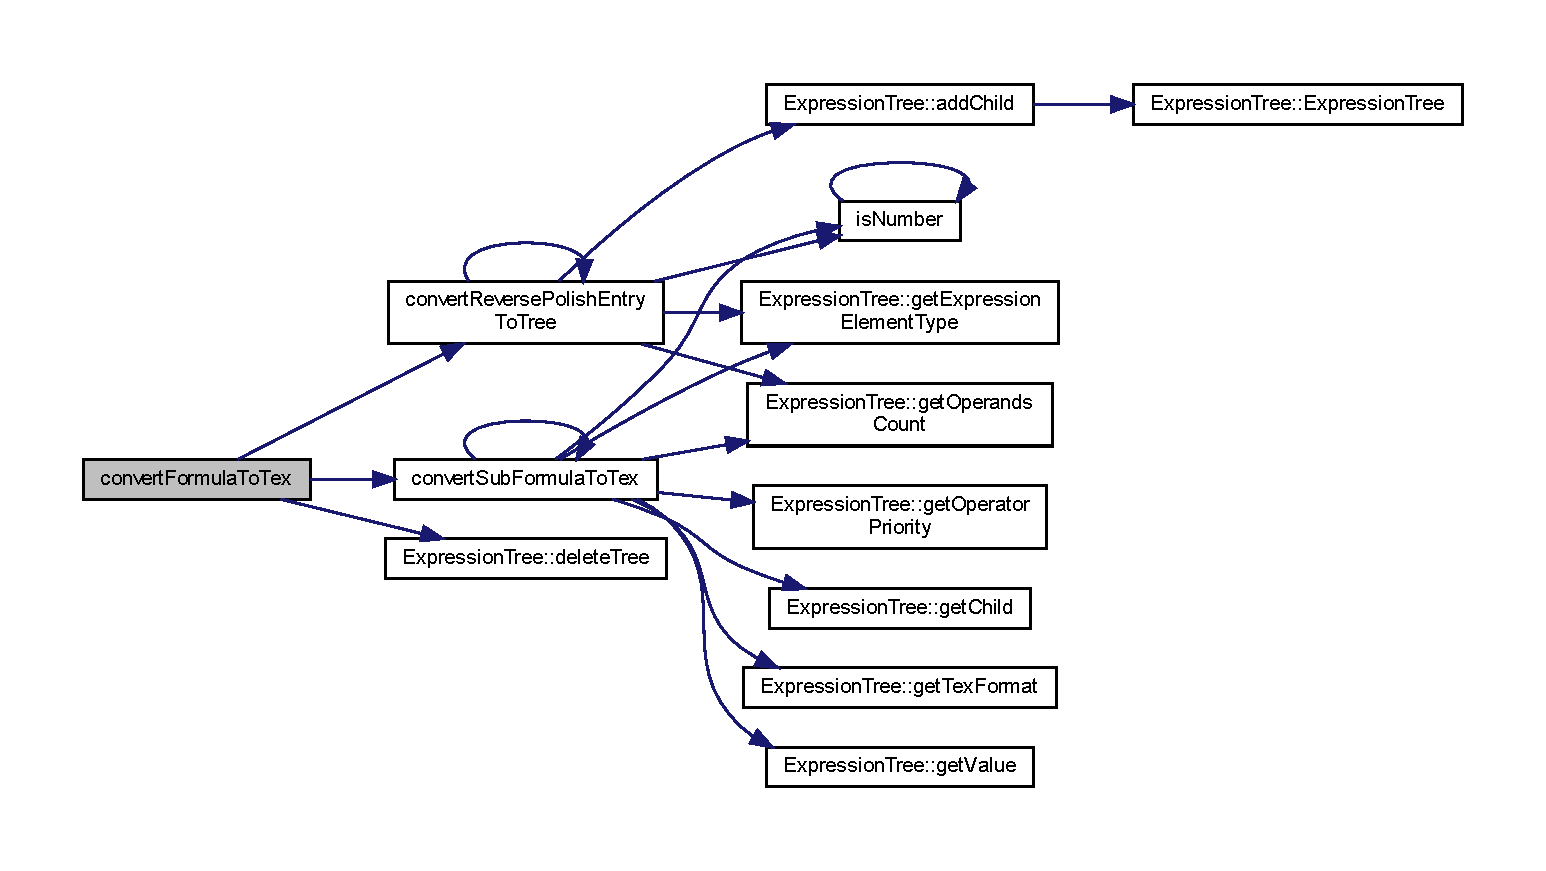
\includegraphics[width=350pt]{convert_tree_to_t_e_x_8h_aec3525860ad5d5b05c0fd16270b606d7_cgraph}
\end{center}
\end{figure}
Граф вызова функции\+:\nopagebreak
\begin{figure}[H]
\begin{center}
\leavevmode
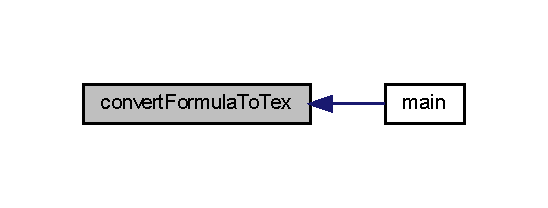
\includegraphics[width=263pt]{convert_tree_to_t_e_x_8h_aec3525860ad5d5b05c0fd16270b606d7_icgraph}
\end{center}
\end{figure}
\mbox{\Hypertarget{convert_tree_to_t_e_x_8h_a4484ae20417cae4ad61d6319cdf03f68}\label{convert_tree_to_t_e_x_8h_a4484ae20417cae4ad61d6319cdf03f68}} 
\index{convert\+Tree\+To\+T\+E\+X.\+h@{convert\+Tree\+To\+T\+E\+X.\+h}!convert\+Reverse\+Polish\+Entry\+To\+Tree@{convert\+Reverse\+Polish\+Entry\+To\+Tree}}
\index{convert\+Reverse\+Polish\+Entry\+To\+Tree@{convert\+Reverse\+Polish\+Entry\+To\+Tree}!convert\+Tree\+To\+T\+E\+X.\+h@{convert\+Tree\+To\+T\+E\+X.\+h}}
\subsubsection{\texorpdfstring{convert\+Reverse\+Polish\+Entry\+To\+Tree()}{convertReversePolishEntryToTree()}}
{\footnotesize\ttfamily \mbox{\hyperlink{class_expression_tree}{Expression\+Tree}}$\ast$ convert\+Reverse\+Polish\+Entry\+To\+Tree (\begin{DoxyParamCaption}\item[{vector$<$ string $>$ \&}]{reverse\+Polish\+Entry\+Elements }\end{DoxyParamCaption})}



Конвертировать обратную польскую запись в дерево выражений 


\begin{DoxyParams}[1]{Аргументы}
\mbox{\tt in}  & {\em reverse\+Polish\+Entry\+Elements} & -\/ вектор элементов обратной польской записи \\
\hline
\end{DoxyParams}
\begin{DoxyReturn}{Возвращает}
указатель на вершину дерева выражений 
\end{DoxyReturn}

\begin{DoxyExceptions}{Исключения}
{\em L\+A\+C\+K\+\_\+\+O\+F\+\_\+\+O\+P\+E\+R\+A\+N\+D\+S\+\_\+\+E\+X\+C\+E\+P\+T\+I\+ON} & -\/ количество операндов для оператора недостаточно \\
\hline
{\em I\+N\+C\+O\+R\+R\+E\+C\+T\+\_\+\+D\+I\+A\+P\+O\+S\+O\+N\+\_\+\+E\+X\+C\+E\+P\+T\+I\+ON} & -\/ количество значащих цифр больше 20 \\
\hline
{\em I\+N\+C\+O\+R\+R\+E\+C\+T\+\_\+\+V\+A\+L\+\_\+\+F\+O\+R\+M\+A\+T\+\_\+\+E\+X\+C\+E\+P\+T\+I\+ON} & -\/ в обратной польской записи есть неопознанный элемент \\
\hline
\end{DoxyExceptions}
Граф вызовов\+:\nopagebreak
\begin{figure}[H]
\begin{center}
\leavevmode
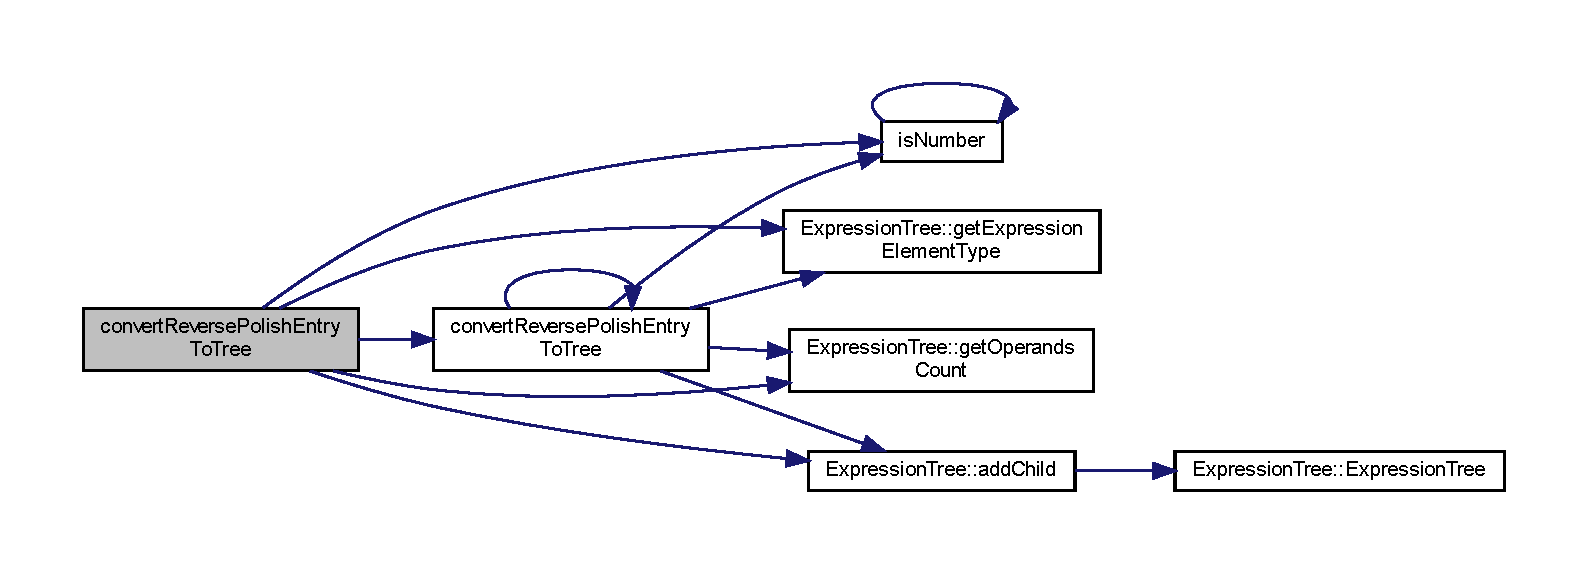
\includegraphics[width=350pt]{convert_tree_to_t_e_x_8h_a4484ae20417cae4ad61d6319cdf03f68_cgraph}
\end{center}
\end{figure}
Граф вызова функции\+:\nopagebreak
\begin{figure}[H]
\begin{center}
\leavevmode
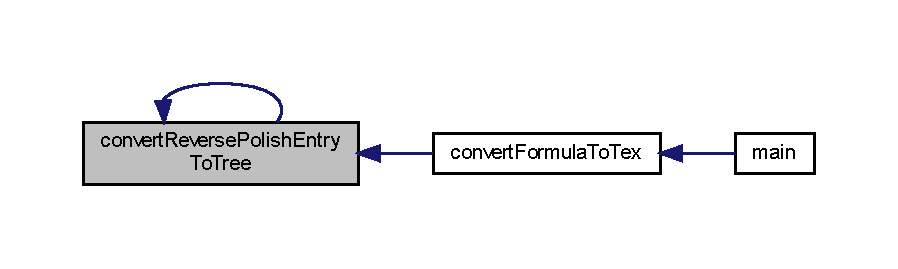
\includegraphics[width=350pt]{convert_tree_to_t_e_x_8h_a4484ae20417cae4ad61d6319cdf03f68_icgraph}
\end{center}
\end{figure}
\mbox{\Hypertarget{convert_tree_to_t_e_x_8h_acccbe3becd02b6dee976c55008082244}\label{convert_tree_to_t_e_x_8h_acccbe3becd02b6dee976c55008082244}} 
\index{convert\+Tree\+To\+T\+E\+X.\+h@{convert\+Tree\+To\+T\+E\+X.\+h}!convert\+Sub\+Formula\+To\+Tex@{convert\+Sub\+Formula\+To\+Tex}}
\index{convert\+Sub\+Formula\+To\+Tex@{convert\+Sub\+Formula\+To\+Tex}!convert\+Tree\+To\+T\+E\+X.\+h@{convert\+Tree\+To\+T\+E\+X.\+h}}
\subsubsection{\texorpdfstring{convert\+Sub\+Formula\+To\+Tex()}{convertSubFormulaToTex()}}
{\footnotesize\ttfamily string convert\+Sub\+Formula\+To\+Tex (\begin{DoxyParamCaption}\item[{\mbox{\hyperlink{class_expression_tree}{Expression\+Tree}} $\ast$}]{current,  }\item[{int \&}]{cur\+Priority }\end{DoxyParamCaption})}



Конвертировать подформулу в tex-\/формулу 


\begin{DoxyParams}[1]{Аргументы}
\mbox{\tt in}  & {\em current} & -\/ вершина дерева выражений \\
\hline
\mbox{\tt out}  & {\em cur\+Priority} & -\/ приоритет вершины \\
\hline
\end{DoxyParams}
\begin{DoxyReturn}{Возвращает}
-\/ tex-\/формула 
\end{DoxyReturn}
Граф вызовов\+:\nopagebreak
\begin{figure}[H]
\begin{center}
\leavevmode
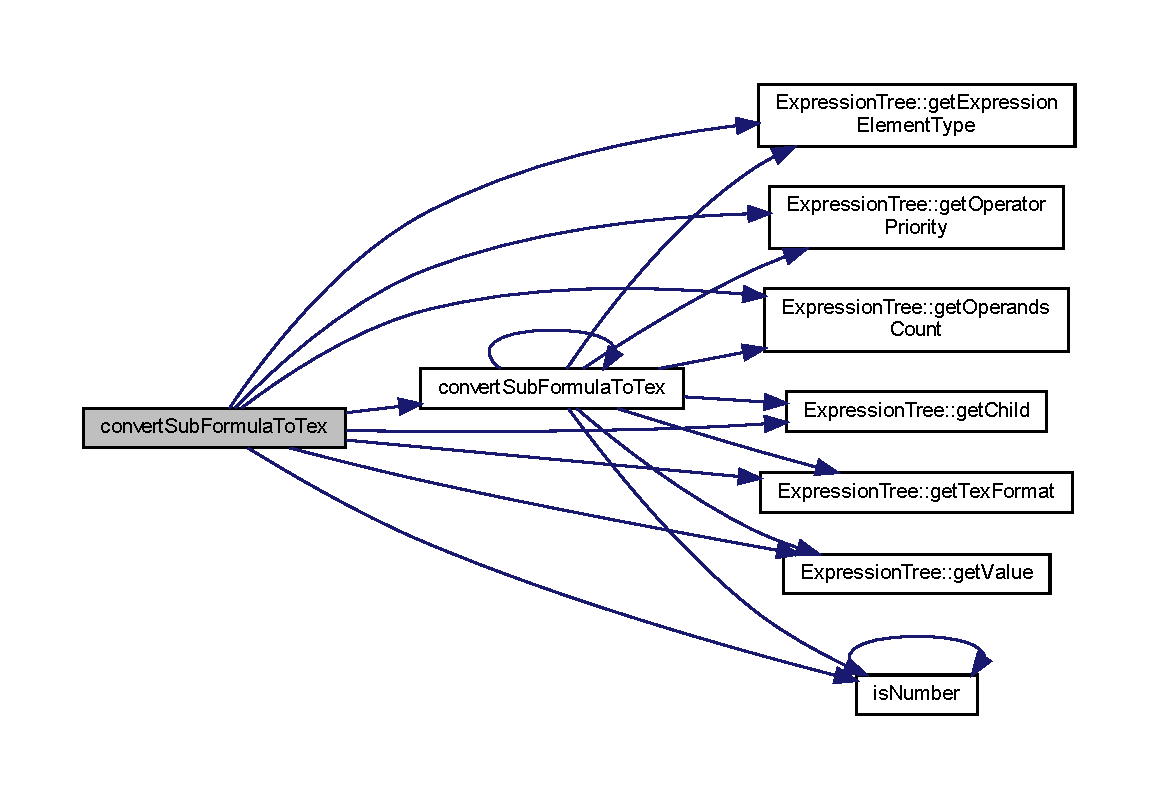
\includegraphics[width=350pt]{convert_tree_to_t_e_x_8h_acccbe3becd02b6dee976c55008082244_cgraph}
\end{center}
\end{figure}
Граф вызова функции\+:\nopagebreak
\begin{figure}[H]
\begin{center}
\leavevmode
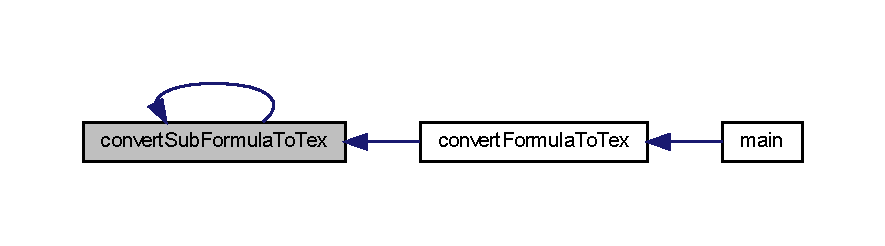
\includegraphics[width=350pt]{convert_tree_to_t_e_x_8h_acccbe3becd02b6dee976c55008082244_icgraph}
\end{center}
\end{figure}

\hypertarget{_expression_tree_8cpp}{}\section{Файл Expression\+Tree.\+cpp}
\label{_expression_tree_8cpp}\index{Expression\+Tree.\+cpp@{Expression\+Tree.\+cpp}}


Файл содержит реализации конструкторов, деструктора, а также методов дерева выражений  


{\ttfamily \#include \char`\"{}Expression\+Tree.\+h\char`\"{}}\newline


\subsection{Подробное описание}
Файл содержит реализации конструкторов, деструктора, а также методов дерева выражений 


\hypertarget{_expression_tree_8h}{}\section{Файл Expression\+Tree.\+h}
\label{_expression_tree_8h}\index{Expression\+Tree.\+h@{Expression\+Tree.\+h}}


Файл содержит перечисление типов элементов обратной польской записи, а также класс дерева выражений  


{\ttfamily \#include \char`\"{}Convert\+To\+T\+E\+X.\+h\char`\"{}}\newline
{\ttfamily \#include $<$iostream$>$}\newline
\subsection*{Классы}
\begin{DoxyCompactItemize}
\item 
class \mbox{\hyperlink{class_expression_tree}{Expression\+Tree}}
\begin{DoxyCompactList}\small\item\em Дерево выражений \end{DoxyCompactList}\end{DoxyCompactItemize}
\subsection*{Перечисления}
\begin{DoxyCompactItemize}
\item 
enum \mbox{\hyperlink{_expression_tree_8h_a3773a0b5484dde6ff527a03ae3b28b75}{Expression\+Element\+Type}} \{ \newline
\mbox{\hyperlink{_expression_tree_8h_a3773a0b5484dde6ff527a03ae3b28b75a12a90dfe20486bbe3e075afcd19ef2d0}{N\+U\+M\+B\+ER}}, 
\mbox{\hyperlink{_expression_tree_8h_a3773a0b5484dde6ff527a03ae3b28b75af68346ce0bfce7ab2ca0a240f5132863}{V\+AR}}, 
\mbox{\hyperlink{_expression_tree_8h_a3773a0b5484dde6ff527a03ae3b28b75a6411d9d6073252e4d316493506bbb979}{O\+P\+E\+R\+A\+T\+OR}}, 
\mbox{\hyperlink{_expression_tree_8h_a3773a0b5484dde6ff527a03ae3b28b75a6d65e44f3c0ee494183303bf1570c364}{G\+R\+E\+E\+K\+L\+E\+T\+T\+ER}}, 
\newline
\mbox{\hyperlink{_expression_tree_8h_a3773a0b5484dde6ff527a03ae3b28b75a605159e8a4c32319fd69b5d151369d93}{U\+N\+D\+E\+F\+I\+N\+ED}}
 \}
\begin{DoxyCompactList}\small\item\em Типы элементов обратной польской записи \end{DoxyCompactList}\end{DoxyCompactItemize}


\subsection{Подробное описание}
Файл содержит перечисление типов элементов обратной польской записи, а также класс дерева выражений 

Данный файл содержит класс дерева выражений с объявлеными методами, конструкторами, а также перечисление типов элементов обратной польской записи 

\subsection{Перечисления}
\mbox{\Hypertarget{_expression_tree_8h_a3773a0b5484dde6ff527a03ae3b28b75}\label{_expression_tree_8h_a3773a0b5484dde6ff527a03ae3b28b75}} 
\index{Expression\+Tree.\+h@{Expression\+Tree.\+h}!Expression\+Element\+Type@{Expression\+Element\+Type}}
\index{Expression\+Element\+Type@{Expression\+Element\+Type}!Expression\+Tree.\+h@{Expression\+Tree.\+h}}
\subsubsection{\texorpdfstring{Expression\+Element\+Type}{ExpressionElementType}}
{\footnotesize\ttfamily enum \mbox{\hyperlink{_expression_tree_8h_a3773a0b5484dde6ff527a03ae3b28b75}{Expression\+Element\+Type}}}



Типы элементов обратной польской записи 

\begin{DoxyEnumFields}{Элементы перечислений}
\raisebox{\heightof{T}}[0pt][0pt]{\index{N\+U\+M\+B\+ER@{N\+U\+M\+B\+ER}!Expression\+Tree.\+h@{Expression\+Tree.\+h}}\index{Expression\+Tree.\+h@{Expression\+Tree.\+h}!N\+U\+M\+B\+ER@{N\+U\+M\+B\+ER}}}\mbox{\Hypertarget{_expression_tree_8h_a3773a0b5484dde6ff527a03ae3b28b75a12a90dfe20486bbe3e075afcd19ef2d0}\label{_expression_tree_8h_a3773a0b5484dde6ff527a03ae3b28b75a12a90dfe20486bbe3e075afcd19ef2d0}} 
N\+U\+M\+B\+ER&Число \\
\hline

\raisebox{\heightof{T}}[0pt][0pt]{\index{V\+AR@{V\+AR}!Expression\+Tree.\+h@{Expression\+Tree.\+h}}\index{Expression\+Tree.\+h@{Expression\+Tree.\+h}!V\+AR@{V\+AR}}}\mbox{\Hypertarget{_expression_tree_8h_a3773a0b5484dde6ff527a03ae3b28b75af68346ce0bfce7ab2ca0a240f5132863}\label{_expression_tree_8h_a3773a0b5484dde6ff527a03ae3b28b75af68346ce0bfce7ab2ca0a240f5132863}} 
V\+AR&Переменная \\
\hline

\raisebox{\heightof{T}}[0pt][0pt]{\index{O\+P\+E\+R\+A\+T\+OR@{O\+P\+E\+R\+A\+T\+OR}!Expression\+Tree.\+h@{Expression\+Tree.\+h}}\index{Expression\+Tree.\+h@{Expression\+Tree.\+h}!O\+P\+E\+R\+A\+T\+OR@{O\+P\+E\+R\+A\+T\+OR}}}\mbox{\Hypertarget{_expression_tree_8h_a3773a0b5484dde6ff527a03ae3b28b75a6411d9d6073252e4d316493506bbb979}\label{_expression_tree_8h_a3773a0b5484dde6ff527a03ae3b28b75a6411d9d6073252e4d316493506bbb979}} 
O\+P\+E\+R\+A\+T\+OR&Оператор \\
\hline

\raisebox{\heightof{T}}[0pt][0pt]{\index{G\+R\+E\+E\+K\+L\+E\+T\+T\+ER@{G\+R\+E\+E\+K\+L\+E\+T\+T\+ER}!Expression\+Tree.\+h@{Expression\+Tree.\+h}}\index{Expression\+Tree.\+h@{Expression\+Tree.\+h}!G\+R\+E\+E\+K\+L\+E\+T\+T\+ER@{G\+R\+E\+E\+K\+L\+E\+T\+T\+ER}}}\mbox{\Hypertarget{_expression_tree_8h_a3773a0b5484dde6ff527a03ae3b28b75a6d65e44f3c0ee494183303bf1570c364}\label{_expression_tree_8h_a3773a0b5484dde6ff527a03ae3b28b75a6d65e44f3c0ee494183303bf1570c364}} 
G\+R\+E\+E\+K\+L\+E\+T\+T\+ER&Греческая буква \\
\hline

\raisebox{\heightof{T}}[0pt][0pt]{\index{U\+N\+D\+E\+F\+I\+N\+ED@{U\+N\+D\+E\+F\+I\+N\+ED}!Expression\+Tree.\+h@{Expression\+Tree.\+h}}\index{Expression\+Tree.\+h@{Expression\+Tree.\+h}!U\+N\+D\+E\+F\+I\+N\+ED@{U\+N\+D\+E\+F\+I\+N\+ED}}}\mbox{\Hypertarget{_expression_tree_8h_a3773a0b5484dde6ff527a03ae3b28b75a605159e8a4c32319fd69b5d151369d93}\label{_expression_tree_8h_a3773a0b5484dde6ff527a03ae3b28b75a605159e8a4c32319fd69b5d151369d93}} 
U\+N\+D\+E\+F\+I\+N\+ED&Неопределенный элемент обратной польской записи \\
\hline

\end{DoxyEnumFields}

\hypertarget{_soft_q_a___chupinin__11_8cpp}{}\section{Файл Soft\+Q\+A\+\_\+\+Chupinin\+\_\+11.\+cpp}
\label{_soft_q_a___chupinin__11_8cpp}\index{Soft\+Q\+A\+\_\+\+Chupinin\+\_\+11.\+cpp@{Soft\+Q\+A\+\_\+\+Chupinin\+\_\+11.\+cpp}}
{\ttfamily \#include $<$iostream$>$}\newline
{\ttfamily \#include \char`\"{}convert\+Tree\+To\+T\+E\+X.\+h\char`\"{}}\newline
{\ttfamily \#include $<$string$>$}\newline
{\ttfamily \#include $<$boost/algorithm/string.\+hpp$>$}\newline
\subsection*{Макросы}
\begin{DoxyCompactItemize}
\item 
\#define \mbox{\hyperlink{_soft_q_a___chupinin__11_8cpp_af08ec37a8c99d747fb60fa15bc28678b}{\+\_\+\+C\+R\+T\+\_\+\+S\+E\+C\+U\+R\+E\+\_\+\+N\+O\+\_\+\+W\+A\+R\+N\+I\+N\+GS}}
\end{DoxyCompactItemize}
\subsection*{Функции}
\begin{DoxyCompactItemize}
\item 
int \mbox{\hyperlink{_soft_q_a___chupinin__11_8cpp_a0ddf1224851353fc92bfbff6f499fa97}{main}} (int argc, char $\ast$argv\mbox{[}$\,$\mbox{]})
\end{DoxyCompactItemize}


\subsection{Макросы}
\mbox{\Hypertarget{_soft_q_a___chupinin__11_8cpp_af08ec37a8c99d747fb60fa15bc28678b}\label{_soft_q_a___chupinin__11_8cpp_af08ec37a8c99d747fb60fa15bc28678b}} 
\index{Soft\+Q\+A\+\_\+\+Chupinin\+\_\+11.\+cpp@{Soft\+Q\+A\+\_\+\+Chupinin\+\_\+11.\+cpp}!\+\_\+\+C\+R\+T\+\_\+\+S\+E\+C\+U\+R\+E\+\_\+\+N\+O\+\_\+\+W\+A\+R\+N\+I\+N\+GS@{\+\_\+\+C\+R\+T\+\_\+\+S\+E\+C\+U\+R\+E\+\_\+\+N\+O\+\_\+\+W\+A\+R\+N\+I\+N\+GS}}
\index{\+\_\+\+C\+R\+T\+\_\+\+S\+E\+C\+U\+R\+E\+\_\+\+N\+O\+\_\+\+W\+A\+R\+N\+I\+N\+GS@{\+\_\+\+C\+R\+T\+\_\+\+S\+E\+C\+U\+R\+E\+\_\+\+N\+O\+\_\+\+W\+A\+R\+N\+I\+N\+GS}!Soft\+Q\+A\+\_\+\+Chupinin\+\_\+11.\+cpp@{Soft\+Q\+A\+\_\+\+Chupinin\+\_\+11.\+cpp}}
\subsubsection{\texorpdfstring{\+\_\+\+C\+R\+T\+\_\+\+S\+E\+C\+U\+R\+E\+\_\+\+N\+O\+\_\+\+W\+A\+R\+N\+I\+N\+GS}{\_CRT\_SECURE\_NO\_WARNINGS}}
{\footnotesize\ttfamily \#define \+\_\+\+C\+R\+T\+\_\+\+S\+E\+C\+U\+R\+E\+\_\+\+N\+O\+\_\+\+W\+A\+R\+N\+I\+N\+GS}



\subsection{Функции}
\mbox{\Hypertarget{_soft_q_a___chupinin__11_8cpp_a0ddf1224851353fc92bfbff6f499fa97}\label{_soft_q_a___chupinin__11_8cpp_a0ddf1224851353fc92bfbff6f499fa97}} 
\index{Soft\+Q\+A\+\_\+\+Chupinin\+\_\+11.\+cpp@{Soft\+Q\+A\+\_\+\+Chupinin\+\_\+11.\+cpp}!main@{main}}
\index{main@{main}!Soft\+Q\+A\+\_\+\+Chupinin\+\_\+11.\+cpp@{Soft\+Q\+A\+\_\+\+Chupinin\+\_\+11.\+cpp}}
\subsubsection{\texorpdfstring{main()}{main()}}
{\footnotesize\ttfamily int main (\begin{DoxyParamCaption}\item[{int}]{argc,  }\item[{char $\ast$}]{argv\mbox{[}$\,$\mbox{]} }\end{DoxyParamCaption})}

Граф вызовов\+:\nopagebreak
\begin{figure}[H]
\begin{center}
\leavevmode
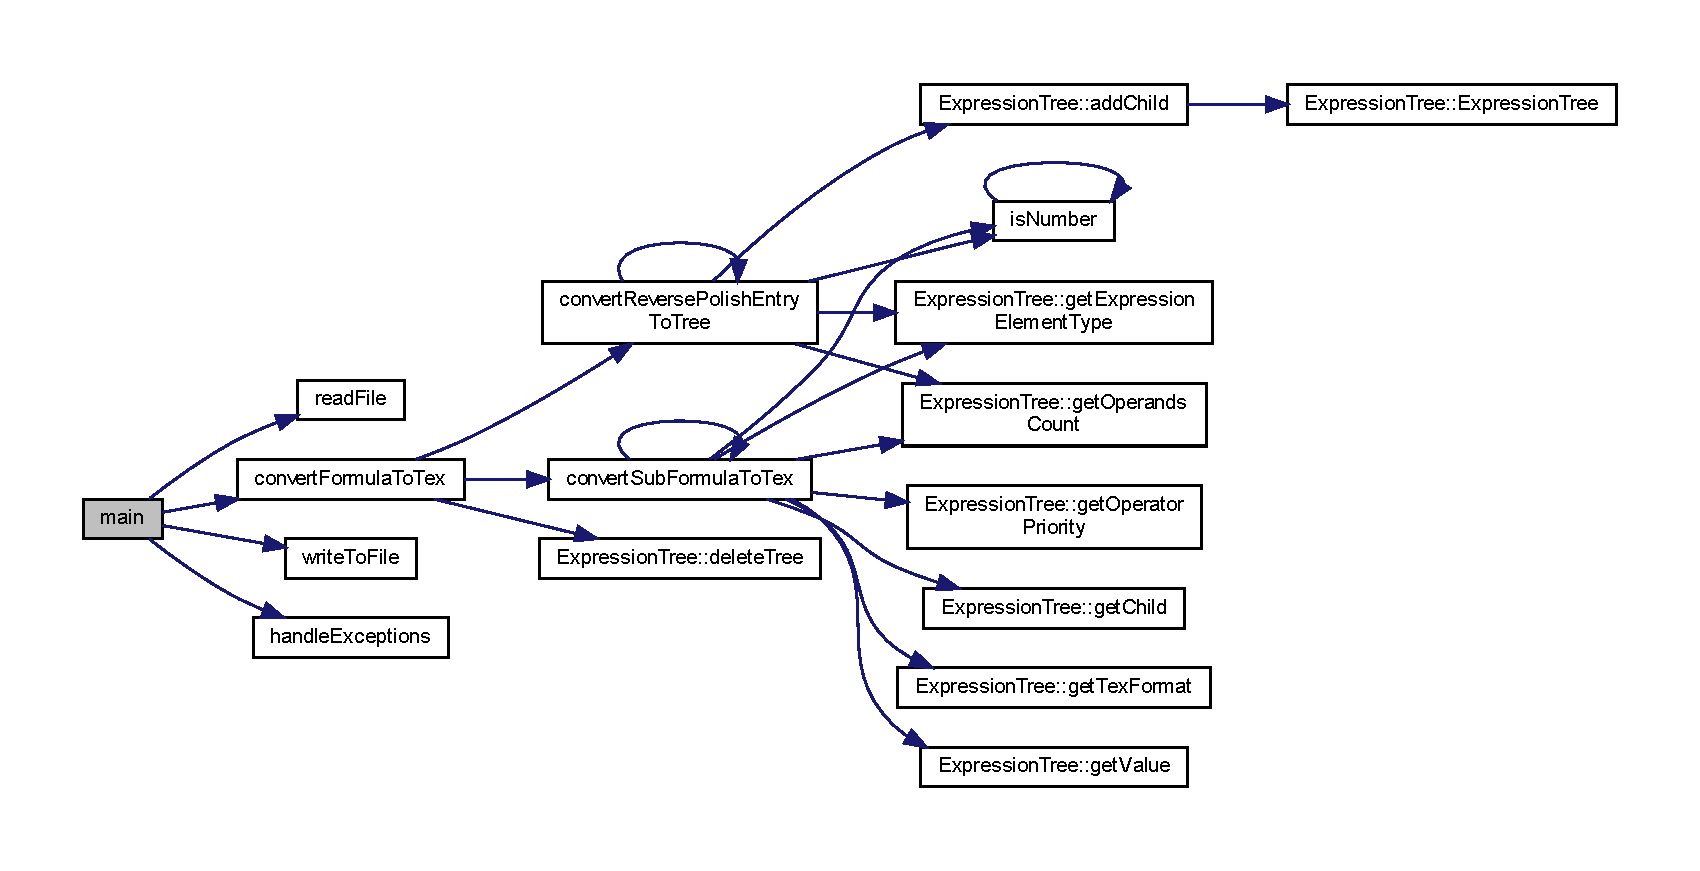
\includegraphics[width=350pt]{_soft_q_a___chupinin__11_8cpp_a0ddf1224851353fc92bfbff6f499fa97_cgraph}
\end{center}
\end{figure}

%--- End generated contents ---

% Index
\backmatter
\newpage
\phantomsection
\clearemptydoublepage
\addcontentsline{toc}{chapter}{Алфавитный указатель}
\printindex

\end{document}
